\documentclass[11pt,letterpaper]{article}

\usepackage{graphicx,float}
\usepackage{caption}  % "subfig" & "subcaption" requires "caption" package
\usepackage[labelformat=empty]{subfig}  % "=empty": no sub-caption
\usepackage{amsmath,natbib,bm,url}
\usepackage{amssymb,amsfonts}
\usepackage{microtype} % character protrusion, font expansion, adjustment of interword spacing, etc.
\usepackage[top=0.75in,bottom=0.95in,left=0.9in,right=0.9in]{geometry}
\usepackage{hyperref}
\hypersetup{    % See reference: http://en.wikibooks.org/wiki/LaTeX/Hyperlinks
    %    bookmarks=true,         % show bookmarks bar?
    %    unicode=false,          % non-Latin characters in Acrobat's bookmarks
    %    pdftoolbar=true,        % show Acrobat's toolbar?
    %    pdfmenubar=true,        % show Acrobat's menu?
    %    pdffitwindow=false,     % window fit to page when opened
    pdfstartview={FitH},    % fits the width of the page to the window
    %    pdftitle={My Title},    % title
    %    pdfauthor={Shi, Jian},     % author
    %    pdfsubject={My Subject},   % subject of the document
    %    pdfcreator={Shi, Jian},   % creator of the document
    %    pdfproducer={Producer}, % producer of the document
    %    pdfkeywords={keyword1} {key2} {key3}, % list of keywords
    %    pdfnewwindow=true,      % links in new window
    colorlinks=true,       % false: boxed links; true: colored links
    linkcolor=blue,          % color of internal links
    citecolor=blue,        % color of links to bibliography
    %    filecolor=magenta,      % color of file links
    %    urlcolor=cyan           % color of external links
}

\usepackage[nottoc]{tocbibind}  % This package will include bibliography to table of contents
\usepackage{makeidx} % make index

% % % % Paragraph Settings % % % %
\renewcommand{\baselinestretch}{1.20}  % space between lines
\setlength{\parskip}{0.25\baselineskip} % space between paragraphs
%\setlength{\parindent}{0em}   % no indent at the start of paragraph
% % % % % % % % % % % % % % % %

\clubpenalty = 10000   % prevent ``widows'' and ``orphans''
\widowpenalty = 10000  % prevent ``widows'' and ``orphans''

\usepackage{mathptmx}
\usepackage{helvet}

\usepackage{multicol}   % multi-column (usage: \begin{multicols}{2} ...... \end{multicols})
\usepackage{epstopdf}   % When using pdfLaTeX and XeLaTeX, directly converts EPS figure into PDF format

\usepackage{amsmath,amssymb} % necessary for typesetting math formulae


\usepackage{multirow}
\usepackage{wrapfig}

\usepackage{framed}

\graphicspath{ {./figures/} }

\usepackage{color}
\definecolor{lightgray}{gray}{0.83}

\newcommand{\panel}[1]{\colorbox{lightgray}{\textsf{#1}}}

\newcommand{\ein}[1]{~\mathrm{#1}}  % units
\newcommand{\f}[2]{\frac{#1}{#2}}
\newcommand{\xeq}[1]{\stackrel{\;#1}{\cleaders\hbox{=\!}\hfill}\:} % extendible equal sign
\newcommand{\eqdef}{\xeq{\mathrm{def}}}
\newcommand{\la}{\langle}
\newcommand{\ra}{\rangle}
\newcommand{\mrm}{\mathrm}

\setcounter{tocdepth}{3}

\usepackage{makecell}


\title{\textbf{\textsf{\huge{SeismoSoil User Manual,} \LARGE{v1.3}}}}
\date{}


\begin{document}
  \maketitle
  \thispagestyle{empty}    % No page number on the first page
  \vspace{-10pt}

SeismoSoil is a site-specific response analysis software application, which performs 1-D linear elastic, equivalent linear, and nonlinear site response analyses.
    

\begin{framed}
	\begin{center}
		\textbf{By downloading or using this software, you acknowledge acceptance of the following DISCLAIMER OF WARRANTY AND LIABILITY:}
	\end{center}
	
	{\sffamily
			THIS SOFTWARE AND/OR RELATED MATERIALS ARE PROVIDED ``AS-IS'' WITHOUT WARRANTY OF ANY KIND. WE MAKE NO WARRANTIES, EXPRESS OR IMPLIED, THAT THEY ARE FREE OF ERROR, OR ARE CONSISTENT WITH ANY PARTICULAR BUILDING CODES AND/OR STANDARDS, OR ARE SUITABLE FOR A PARTICULAR USE OR PURPOSE OR FOR ANY PURPOSE WHATSOEVER, HOWEVER USED.
			
			IN NO EVENT SHALL THE CALIFORNIA INSTITUTE OF TECHNOLOGY OR THE AUTHORS OF THIS SOFTWARE BE LIABLE FOR ANY DIRECT, INDIRECT, INCIDENTAL, SPECIAL, EXEMPLARY, OR CONSEQUENTIAL DAMAGES (INCLUDING, BUT NOT LIMITED TO, PROCUREMENT OF SUBSTITUTE GOODS OR SERVICES; LOSS OF USE, DATA, OR PROFITS; DAMAGE TO COMPUTING EQUIPMENT, COMPUTER SYSTEMS, SOFTWARE, OR STORED DIGITAL DATA; OR BUSINESS INTERRUPTION) HOWEVER CAUSED AND ON ANY THEORY OF LIABILITY, WHETHER IN CONTRACT, STRICT LIABILITY, OR TORT (INCLUDING NEGLIGENCE OR OTHERWISE) ARISING IN ANY WAY OUT OF THE USE OF THIS SOFTWARE, EVEN IF ADVISED OF THE POSSIBILITY OF SUCH DAMAGE.
			
			USER BEARS ALL RISK RELATING TO QUALITY AND PERFORMANCE OF THIS SOFTWARE AND/OR RELATED MATERIALS.
			
	}
	
	\vspace{0.5cm}
\end{framed}

\begin{center}
To reference the SeismoSoil software, please use the following format:\\
D.~Asimaki and J.~Shi (2017) ``SeismoSoil User Manual, v1.3''
\end{center}

\begin{center}
	\textcopyright~ 2014--2017, GeoQuake Research Group, California Institute of Technology
\end{center}

\newpage
\tableofcontents

\newpage
\section{Introduction}

SeismoSoil is a one-dimensional (1D) site response analysis simulation and visualization application.

\subsection{Main features}
%The main features of SeismoSoil includes the following:
\begin{itemize}
    \item \textbf{\textsf{Linear analysis}}
        \begin{itemize}
            \item Frequency domain analysis, which performs the most basic and simplest type of analysis, following the Haskell-Thompson formulation \citep{Haskell_1953,Thomson_1950}
            \item Time domain analysis, useful when the ``wrap-around'' phenomenon of Fourier transform is pronounced and needs to be addressed
        \end{itemize}
    \item \textbf{\textsf{Equivalent linear analysis (frequency domain)}}
        \begin{itemize}
            \item Original \cite{Seed_Idriss_1970_techreport} equivalent linear method
            \item Frequency dependent moduli and damping method \citep{Assimaki_Kausel_2002}
        \end{itemize}
    \item \textbf{\textsf{Nonlinear analysis (time domain)}}
        \begin{itemize}
            \item \emph{H2}: modified hyperbolic (MKZ) stress-strain model (\citealp{Matasovic_Vucetic_1993}) + Masing unloading/reloading rule, or
            \item \emph{H4}: MKZ + \cite{Muravskii_2005} unloading/reloading rule (non-Masing)
            \item \emph{EPP}: Elasto-perfectly plastic stress-strain model + Masing unloading/reloading rule
            \item \emph{HH}: Hybrid hyperbolic stress-strain model \citep{Shi_Asimaki_2017} that takes into account soil shear strength + non-Masing rule
        \end{itemize}
    \item \textbf{\textsf{Auto-generation of modulus reduction and damping curves}}
        \begin{itemize}
            \item Generates $G/G_{\text{max}}$ curves conforming to the MKZ model, using empirical formulas proposed by \cite{Darendeli_2001}
            \item Generates damping curves using formulas proposed by \cite{Darendeli_2001}
            \item Generates $G/G_{\text{max}}$ curves conforming to the HH model, using the empirical procedures proposed in \cite{Shi_Asimaki_2017}
        \end{itemize}
    \item \textbf{\textsf{Various tools that aid the simulation of site response}}
        \begin{itemize}
            \item Baseline correction, digital signal filtering
            \item Motion deconvolution, response spectra calculations, etc.
            \item Ground motion format conversion (from PEER and SMC format to two-columns)
        \end{itemize}
    \item \textbf{\textsf{Fast and easy-to-use graphical user interface (GUI)}}
        \begin{itemize}
            \item The GUI is intuitive and self-explanatory
            \item SeismoSoil utilizes parallel computing, enabling fast processing speed even for nonlinear analyses
            \item All input and output data files are in plain text format, allowing easy pre-processing and post-processing in Excel/MATLAB/Python/etc.
            \item Figures generated can be directly saved to hard drive
        \end{itemize}
\end{itemize}

\newpage
\subsection{Functionality structure}

\begin{figure}[H]
\centering
  % Requires \usepackage{graphicx}
  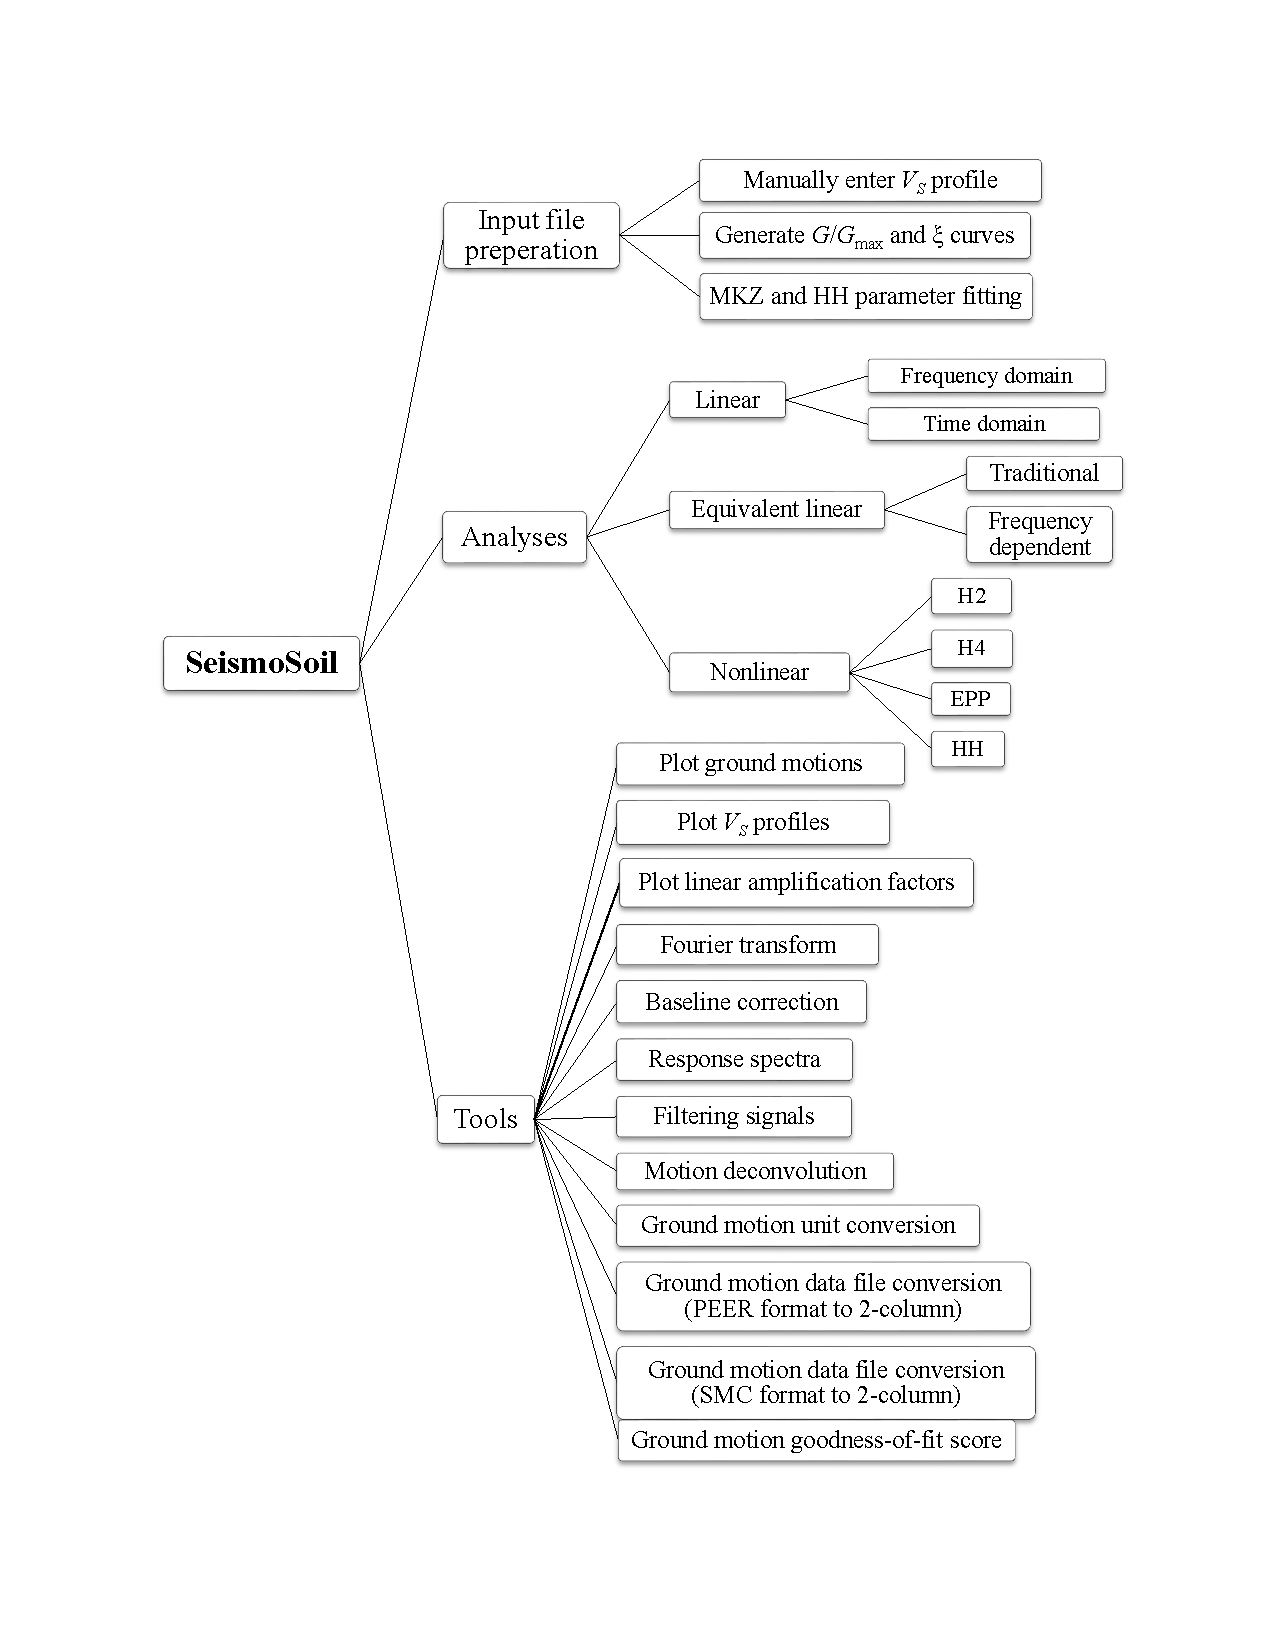
\includegraphics[height=.95\textheight]{functionality_structure.pdf}\\
  %\caption{}\label{}
\end{figure}

%\newpage
\section{Quick tutorial}
\subsection{Installation}

\subsubsection{Windows users}

\begin{enumerate}
	\item Install MATLAB Compiler Runtime (MCR), which can be downloaded from MathWorks website for free\footnote{\href{http://www.mathworks.com/products/compiler/mcr}{\textsf{http://www.mathworks.com/products/compiler/mcr}}}. Please choose \textbf{``R2017b (9.3), 64-bit''}. If your computer has a full MATLAB R2017b (64-bit) installation, you can skip this step.
	
	\item Open {\textsf{{SeismoSoil.exe}}}. (Please keep the other auxiliary files, {\textsf{TDLinear.exe}}, {\textsf{FDEQ.exe}}, {\textsf{NLEPP.exe}}, {\textsf{NLH2.exe}}, {\textsf{NLH4.exe}}, and {\textsf{NLHH.exe}}, in the same directory as {\textsf{{SeismoSoil.exe}}})
\end{enumerate}

\subsubsection{Mac users}

\begin{enumerate}
	\item Install MATLAB Compiler Runtime (MCR), which can be downloaded from MathWorks website for free. Please choose \textbf{``R2017b (9.3), 64-bit''}. If your computer has a full MATLAB R2017b (64-bit) installation, you can skip this step.
    
	\item Place the APP file (the file with the MATLAB icon) in the Applications folder. (This is a must; otherwise there will be strange errors.)
	\item From the Terminal, execute the following (without the quotation marks):\\
	 ``\texttt{/Applications/SeismoSoil.app/Contents/MacOS/applauncher}''. \\(Please start SeismoSoil only from the Terminal. If you open it by double-clicking the icon, some unexpected errors will occur during runtime.)
\end{enumerate}

The system requirement for SeismoSoil is: Windows 7/8/8.1/10 (64-bit) or macOS (64-bit Mavericks or newer), with enough disk space (recommended 4~GB). There is no requirement for minimum CPU and memory, but SeismoSoil runs much faster on more advanced machines (especially with more CPU cores).

The screenshot of the \panel{main} panel of SeismoSoil (shown on the next page) will appear after startup.

\subsection{Input files preparation}

Input file examples are provided in the folder ``Sample Input Files''. Users can start trying SeismoSoil right away using these sample files, or can follow the following paragraphs in this section to learn to prepare new input files.

All input files should be plain text files (such as \textsf{.txt} files). Acceptable column delimiters include spaces, commas, and horizontal tabs, but users should not mix different types of delimiters in a same input file.

The output files generated by SeismoSoil will use horizontal tabs as delimiters.

\begin{figure}[H]
\centering
  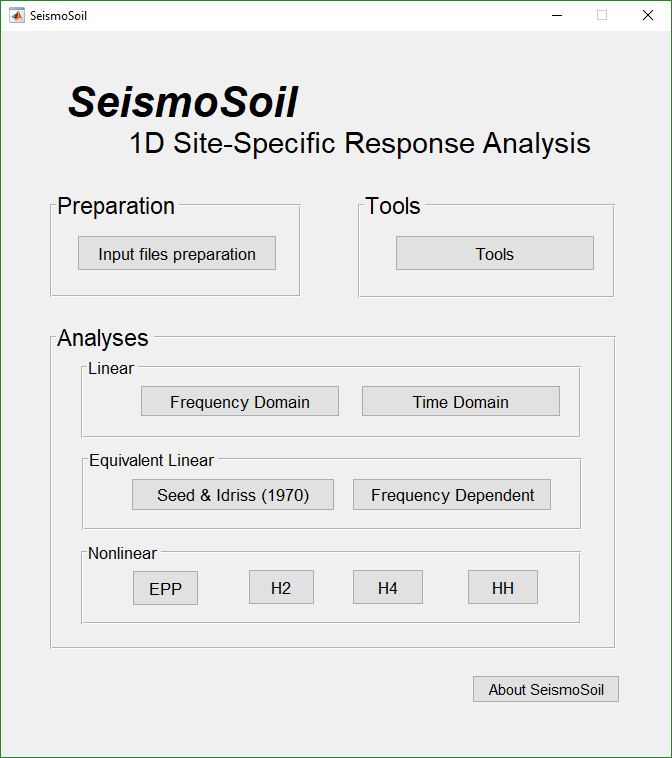
\includegraphics[width=.9\textwidth]{main.png}\\
\end{figure}

\newpage
\subsubsection{Ground motion}\label{sec:motion_file}

Ground motion data files should have exactly two columns---the left column is the time vector in units of seconds, and the right column is the acceleration, in units of $\ein{m/s^2}$, gal ($=1\ein{cm/s^2}$), or $g$ ($=9.81\ein{m/s^2}$). Users can choose their corresponding unit in simulation graphical panels.\footnote{There is a \panel{PEER to 2-column converter} panel under \panel{main}$\rightarrow$\panel{tools}, which converts the~\textsf{.AT2} format used by PEER/NGA database into 2-column format. Similarly, the \panel{SMC to 2-column converter} converts the SMC format into 2-column format.}

\panel{Main}$\rightarrow$\panel{tools}$\rightarrow$\panel{ground motion plotter} provides plots of acceleration time history, as well as velocity and displacement time histories, which are integrated from the acceleration. Arias intensity and RMS acceleration can also be calculated. An example output of the \panel{ground motion plotter} is shown below.

\begin{figure}[H]
\centering
  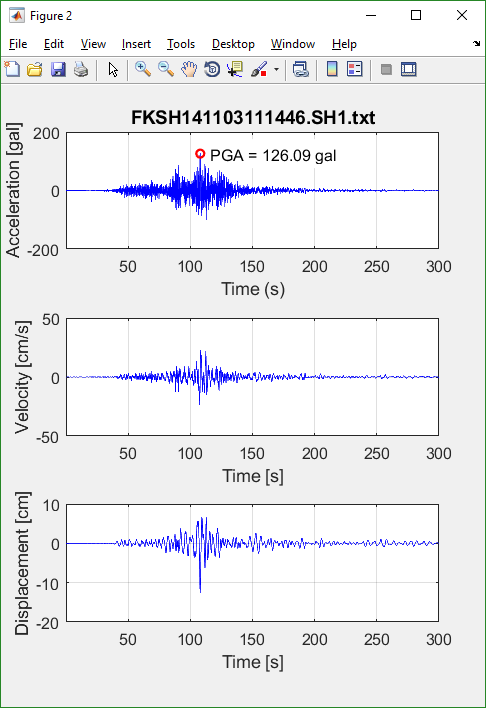
\includegraphics[width=.62\textwidth]{ground_motion_plot.png}\\
\end{figure}

Under \panel{main}$\rightarrow$\panel{tools}, users can also find \panel{signal filter} and \panel{baseline correction}, which filter or baseline-correct the ground motion accelerations; in addition, they can plot the Fourier spectra with \panel{Fourier transform} and elastic response spectra (with any damping ratio value) with \panel{elastic response spectra}. An example of the baseline correction output is shown below. The algorithm of the baseline correction is listed in Section \ref{sec:baseline-correction}.

\begin{figure}[H]
\centering
  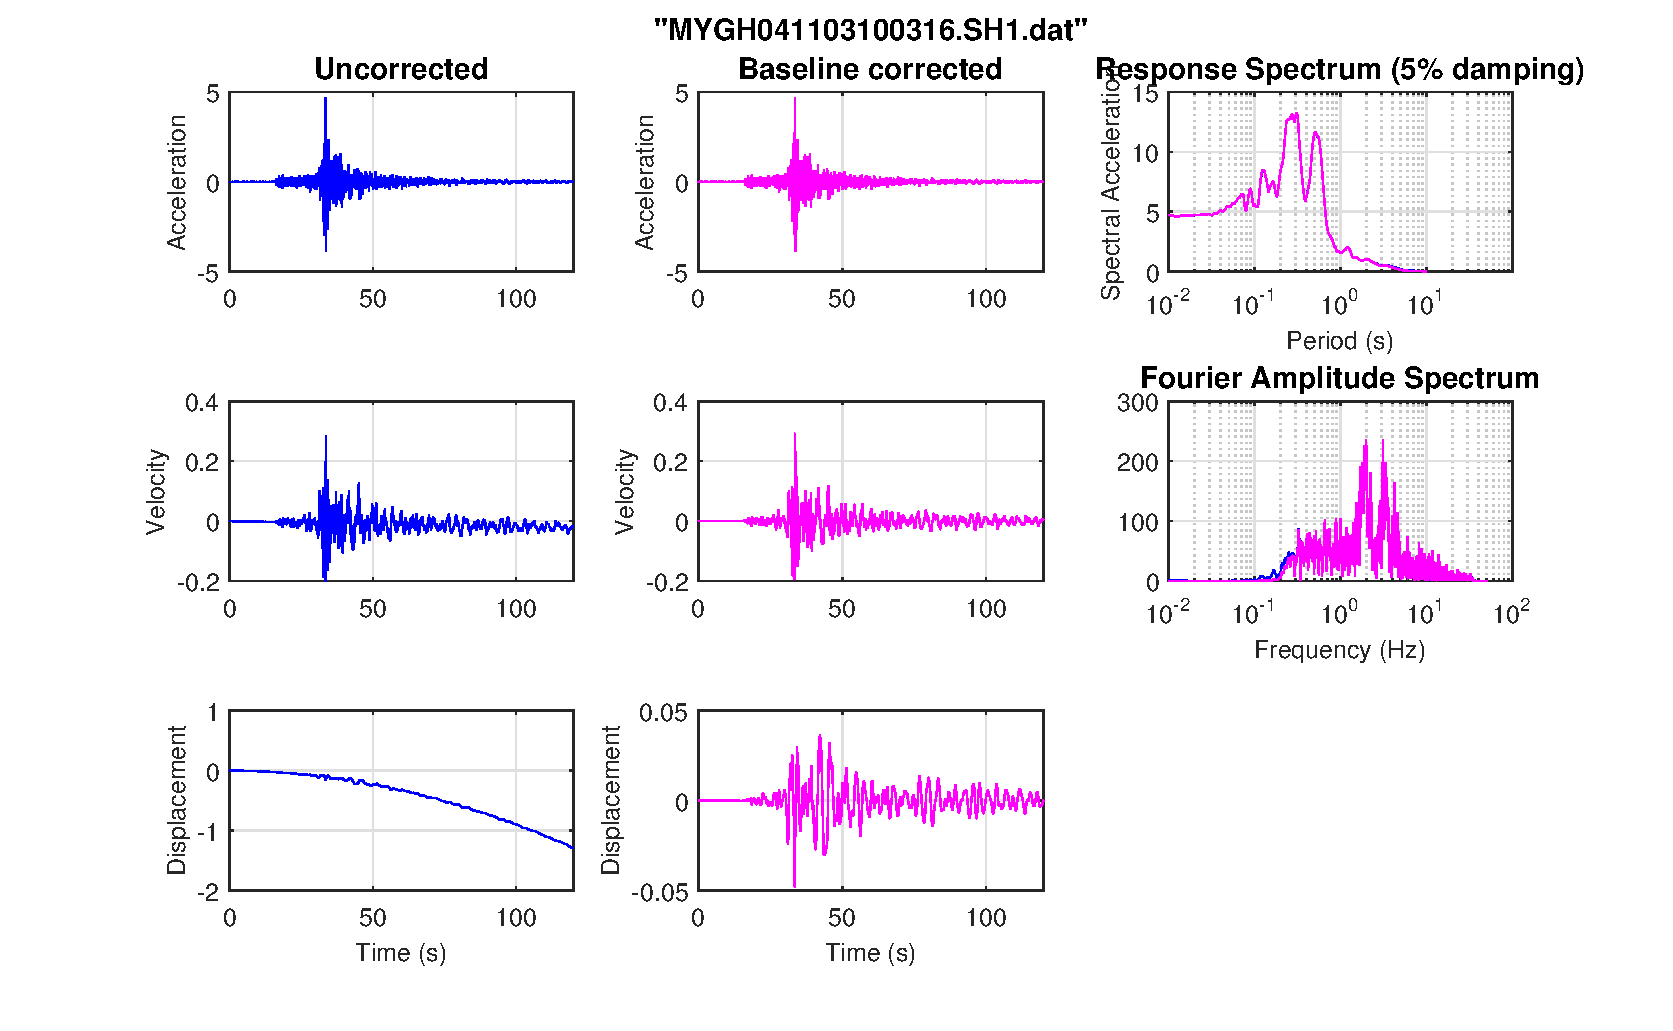
\includegraphics[width=.99\textwidth]{baseline_correction_result_new.pdf}\\
  \label{fig:baseline_result}
\end{figure}

\subsubsection{Shear-wave velocity ($V_S$) profile}\label{sec:soil_profile}

The input file containing the soil property profile should be in the following five-column format:

\begin{figure}[H]
\centering
  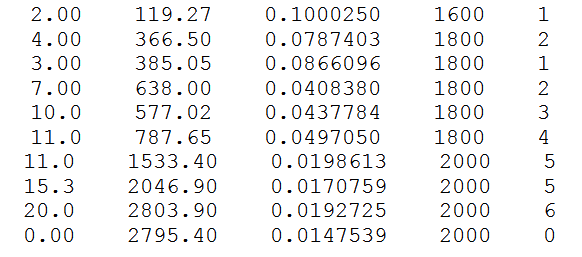
\includegraphics[width=.62\textwidth]{profile_file.png}\\
\end{figure}

The five columns from left to right mean: (1) soil layer thickness (m), (2) shear wave velocity $V_s$ (m/s), (3) low-strain damping ratio, $\xi$, (4) soil mass density, $\rho$, and (5) ``material number'', respectively. The units of $\xi$ can be either \% or unity (i.e., 1), and the unit of $\rho$ can be either $\ein{g/cm^3}$ or $\ein{kg/m^3}$. The users can specify the units of $\xi$ and $\rho$ on the simulation panels, before the analysis starts. The last thickness value \textbf{\emph{should always be 0}}, which indicates the last layer (i.e., the halfspace) has infinite depth. (It can have the same $V_S$, $\xi$, and $\rho$ as the layer above it.)

The fifth column, the ``material number'', should be a series of positive integers, not necessary in a continuous and ascending order, with the exception of the last value, which \emph{should always be 0}. The material number refers to the nonlinear dynamic soil parameters, namely the $G/G_{\max}$ and damping curves. For example, the layers with ``material number''=5 correspond to the 5th set of $G/G_{\max}$ and damping curves in the ``curve file'', which will be explained in Section \ref{sec:curve}.

The soil profile can be manually entered through \panel{main}$\rightarrow$\panel{input files preparation}$\rightarrow$\panel{manually enter Vs profile}. A screenshot of this panel is shown below.  Alternatively, users can prepare the input files in external applications like Excel or Notepad, and save them as plain text files.

\begin{figure}[H]
\centering
  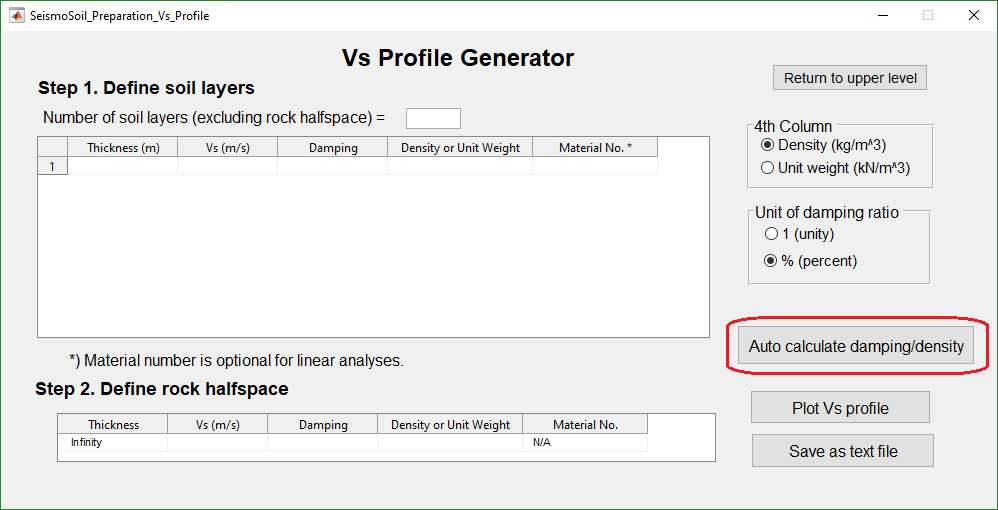
\includegraphics[width=\textwidth]{profile_prepare.png}\\
\end{figure}

The ``Auto calculate damping/density'' button on the panel (in the red box) can generate damping and density for soil layers based on their $V_S$, using the following rules:

\begin{itemize}
    \item Damping ratio $\xi=1/(2Q_S)$, and $Q_S=$
    \begin{itemize}
        \item $0.06V_S$, when $V_S\leqslant1000\ein{m/s}$
        \item $0.04V_S$, when $1000\ein{m/s}< V_S<2000\ein{m/s}$
        \item $0.16V_S$, when $V_S\geqslant 2000\ein{m/s}$
    \end{itemize}
    \item Mass density
    \begin{itemize}
        \item $1.6\ein{g/cm^3}$, when $V_S<200\ein{m/s}$
        \item $1.8\ein{g/cm^3}$, when $200\ein{m/s}\leqslant V_S<800\ein{m/s}$
        \item $2.0\ein{g/cm^3}$, when $V_S\geqslant 800\ein{m/s}$
    \end{itemize}
\end{itemize}

The $Q_S$-$V_S$ correlation above comes from \cite{Archuleta_Liu_2004}.

\subsubsection{Nonlinear soil properties: $G/G_{\max}$ and damping curves}\label{sec:curve}

The two input files mentioned in Sections \ref{sec:motion_file} and \ref{sec:soil_profile} are the only files required for linear site response analysis. For the equivalent linear analysis, dynamic soil properties, namely $G/G_{\max}$ and $\xi$ curves, are required. In SeismoSoil, these properties are specified in a single text file (the ``\textbf{curve file}'').

Below is the format of a ``curve file''. The headers are just for demonstration and should not be included in the actual input file. 

\begin{figure}[H]
\centering
  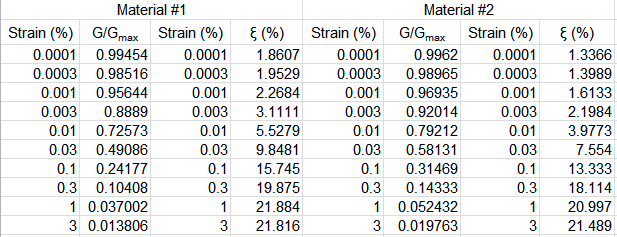
\includegraphics[width=.81\textwidth]{curve_file_format.png}\\
\end{figure}

Each group of four columns corresponds to one material: $G/G_{\max}$ and $\xi$ vs shear strain. Different soil layers can share a same set of $G/G_{\max}$ and $\xi$ curves, and this mapping is provided by the 5th column in the input soil profile file: if the 5th column of a certain layer in the profile file is ``2'', then that layer's $G/G_{\max}$ and $\xi$ curves are the second set of 4 columns in the ``curve file''.

If the user does not know the $G/G_{\max}$ and $\xi$ curves for each layers, SeismoSoil can generate them using the formulas by \cite{Darendeli_2001} (pages 220--272), in \panel{main}$\rightarrow$ \panel{input files preparation}$\rightarrow$\\ \panel{modulus and damping (Darendeli, 2001)}. SeismoSoil chooses the following default values to use in Darendeli's formulas:
\begin{itemize}
\item Total stress analysis (deep groundwater table)
%\item PI (plasticity index) = 20\%
\item OCR: 1.0 (normally consolidated)\footnote{The users are welcome to contact us, if they would like to calculate curves using different OCR, $N$, or $f$ values.}
\item $N$ (number of cycles): 10
\item $f$ = 1 Hz
\end{itemize}

The ground motion, soil profile and dynamic soil properties are the necessary input files for equivalent linear analyses. For nonlinear analyses, the users should also specify the constitutive model parameters, as will be discussed in Sections \ref{sec:para}, \ref{sec:HH_G}, and \ref{sec:HH_x}.

\subsubsection{Nonlinear constitutive model parameters}\label{sec:para}

Apart from the ground motion, soil profile, dynamic curves, the nonlinear analysis in SeismoSoil requires additional information---the constitutive soil parameters. The \emph{H2} nonlinear method requires one file, \textsf{H2\_n.txt}, the \emph{H4} nonlinear method requires two files, \textsf{H4\_G.txt} and \textsf{H4\_x.txt}, and similarly, the \emph{HH} nonlinear method requires two files, \textsf{HH\_G.txt} and \textsf{HH\_x.txt}.  

The format of \textsf{H2\_n.txt}, \textsf{H4\_G.txt}, and \textsf{H4\_x.txt} looks like the figure blow:

\begin{figure}[H]
\centering
  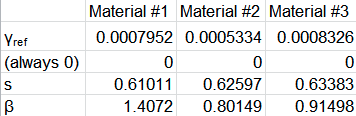
\includegraphics[width=.52\textwidth]{H2_n_format.png}\\
\end{figure}

The file should have exactly 4 rows, and each column of the file corresponds to a set of 4 columns in the ``curve file'', and in the same order as the ``curve file''.

The four rows correspond to the three parameters in the MKZ model: $\gamma_{\text{ref}}$ is the reference strain, and $s$ and $\beta$ are two shape parameters. (Due to legacy reasons, the second row should be all 0's.) The units for them are all SI units (and strains should use the unit of 1, instead of percent).

These three parameters can be obtained by curve-fitting: using the \panel{main}$\rightarrow$\panel{input files preparation}$\rightarrow$ \panel{MKZ (``H2'' or ``H4'') curve fitting} panel (shown in the figure below), which takes a ``curve file'' as input, and generates a \textsf{H2\_n.txt} file (using \emph{H2} curve fitting) or \textsf{H4\_G.txt} and \textsf{H4\_x.txt} files (using \emph{H4} curve fitting).

\begin{figure}[H]
\centering
  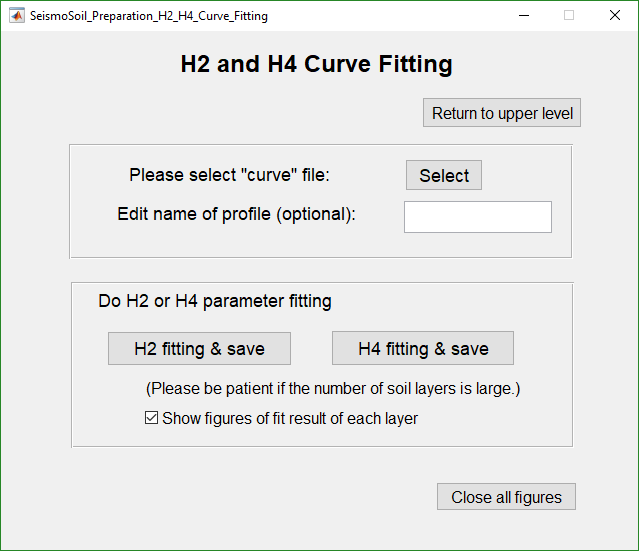
\includegraphics[width=.83\textwidth]{nonlinear_curve_fitting.png}\\
\end{figure}

The format of \textsf{HH\_G.txt} and \textsf{HH\_x.txt} looks like below:

\begin{figure}[H]
    \centering
    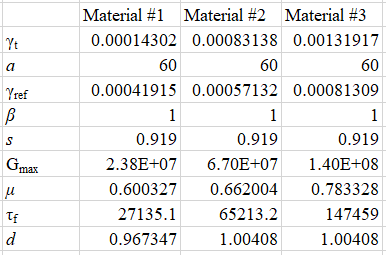
\includegraphics[width=.53\textwidth]{HH_G_format.png}\\
\end{figure}

The file should have exactly 9 rows, and each column of the file corresponds to a set of 4 columns in the ``curve file'', and in the same order as the ``curve file''.

These 9 rows correspond to the 9 parameters of the hybrid hyperbolic (HH) stress-strain model proposed by \cite{Shi_Asimaki_2017}. The units for them are all SI units (and strains should use the unit of 1, instead of percent). The details of the HH model will be explained in Section~\ref{sec:HH_model}, as well as in the original paper \citep{Shi_Asimaki_2017}.

The \textsf{HH\_G.txt} and \textsf{HH\_x.txt} parameters are obtained in different ways, which is explained in Sections \ref{sec:HH_G} and \ref{sec:HH_x} respectively.

\newpage
\subsubsection{Obtaining \textsf{HH\_G} parameters}\label{sec:HH_G}

The \textsf{HH\_G} parameters define the modulus reduction behavior of the HH nonlinear model, and are necessary for performing HH nonlinear analyses. To obtain \textsf{HH\_G} parameters for each soil layers, the user needs at least a shear-wave velocity ($V_S$) profile.

Depending on what information the user has, SeismoSoil handles it differently:

\begin{figure}[H]
    \centering
    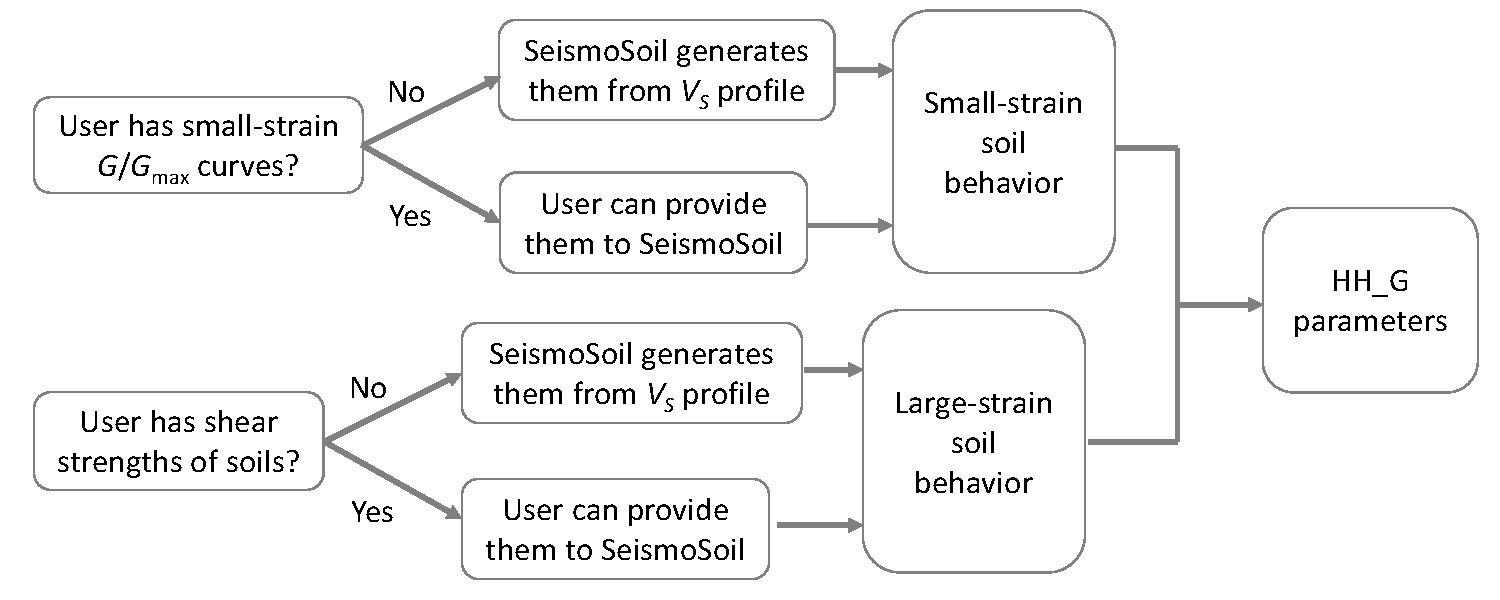
\includegraphics[width=.92\textwidth]{HH_G_decision_tree.pdf}\\
\end{figure}

SeismoSoil performs the procedures above in \panel{main}$\rightarrow$ \panel{input files preparation}$\rightarrow$ \panel{HH\_G}, as shown in the screen shot below.

\begin{figure}[H]
    \centering
    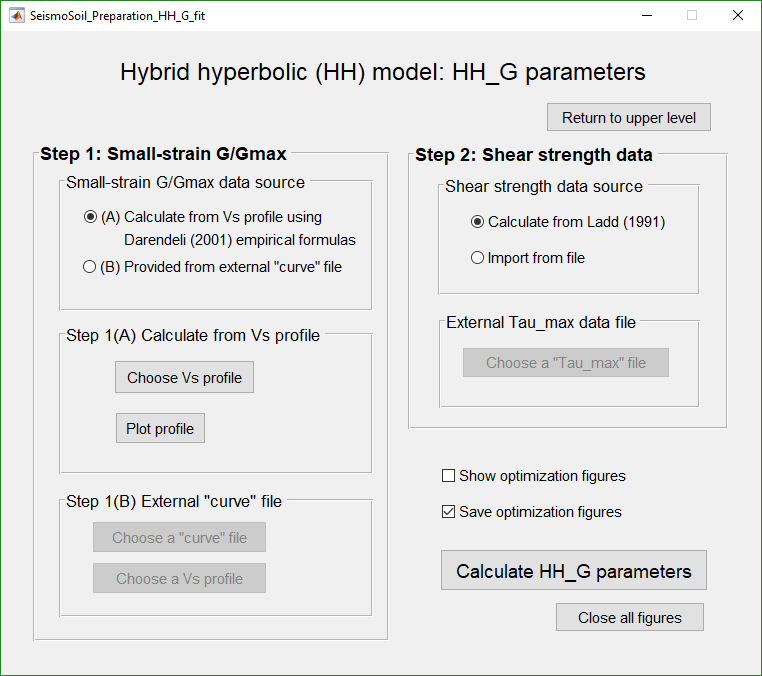
\includegraphics[width=.75\textwidth]{HH_G_fit_panel.png}\\
\end{figure}


\subsubsection{Obtaining \textsf{HH\_x} parameters}\label{sec:HH_x}

The \textsf{HH\_x} parameters defines the damping behavior of the HH nonlinear model, and are necessary for performing HH nonlinear analyses. 

The \textsf{HH\_x} parameters come from curve fitting to damping curves (for each soil layer). If the user does not know the damping for the soils, please follow the procedures in Section~\ref{sec:curve} to generate empirical damping curves.

The \textsf{HH\_x} curve-fit panel is in \panel{main}$\rightarrow$ \panel{input files preparation}$\rightarrow$ \panel{HH\_x}, as shown in the screen shot below. And the user can follow the instructions on the panel. Curve-fitting \textsf{HH\_x} will invoke multiple CPU processors , and will likely take some time to finish (depending on the user's hardware).

\begin{figure}[H]
    \centering
    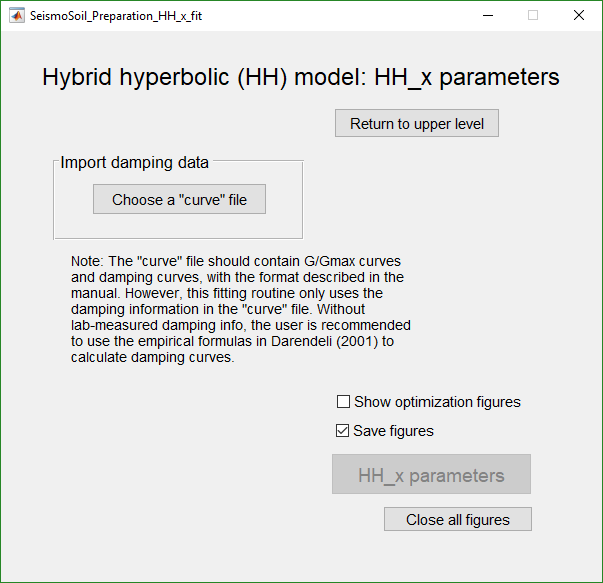
\includegraphics[width=.80\textwidth]{HH_x_fit_panel.png}\\
\end{figure}


\subsubsection{Shear strength}\label{sec:strength}

Shear strength files (usually named \textsf{Tau\_max.txt}) are useful in EPP (elastio-perfectly plastic) nonlinear method as well as HH nonlinear method (if the user knows the shear strength of each soil layer).

The file should have only one column, with each number being the shear strength (unit: Pa) to each soil layer.



\newpage
\subsection{Run simulations}

The input files necessary for different kinds of simulations are summarized below.

\begin{small}
\begin{table}[H]
    \centering
%  \caption{}\label{}
    \begin{tabular}{|c|c|c|c|c|c|c|c|c|c|c|}
         \hline
         & & profile & motion & curve & H2\_n & H4\_G & H4\_x & HH\_G & HH\_x & tau\_max\\
         \hline
        \multirow{2}{*}{Linear} & \makecell{Frequency\\domain} & \checkmark & \checkmark &   &   &  & & & & \\
        \cline{2-11}
         & \makecell{Time\\domain} & \checkmark & \checkmark &   &   & & & & &\\
         \hline
         \multirow{2}{*}{\makecell{Equivalent \\ linear}} & \makecell{Seed \& Idriss\\(1970)} & \checkmark & \checkmark & \checkmark  &   &   & & & &\\
        \cline{2-11}
         & \makecell{Frequency\\dependent} & \checkmark & \checkmark & \checkmark &   &  & & & &\\
         \hline
         \multirow{4}{*}{Nonlinear} & EPP & \checkmark & \checkmark & \checkmark  &   &   & & & & \checkmark\\
         \cline{2-11}
         & H2 & \checkmark & \checkmark & \checkmark  & \checkmark  &   & & & &\\
        \cline{2-11}
         & H4 & \checkmark & \checkmark & \checkmark &   & \checkmark & \checkmark  & & &\\
         \cline{2-11}
         & HH & \checkmark & \checkmark & \checkmark &   &  &  & \checkmark & \checkmark &\\
         \hline
    \end{tabular}
\end{table}
\end{small}


The user interface for linear analysis is shown below. The users can follow ``step 1'' to ``step 3'' on the panel and import the corresponding data. And then the users can click \textsf{Start} to start the calculation. Time-domain and frequency-domain linear methods have the same user interface.

\begin{figure}[H]
\centering
  % Requires \usepackage{graphicx}
  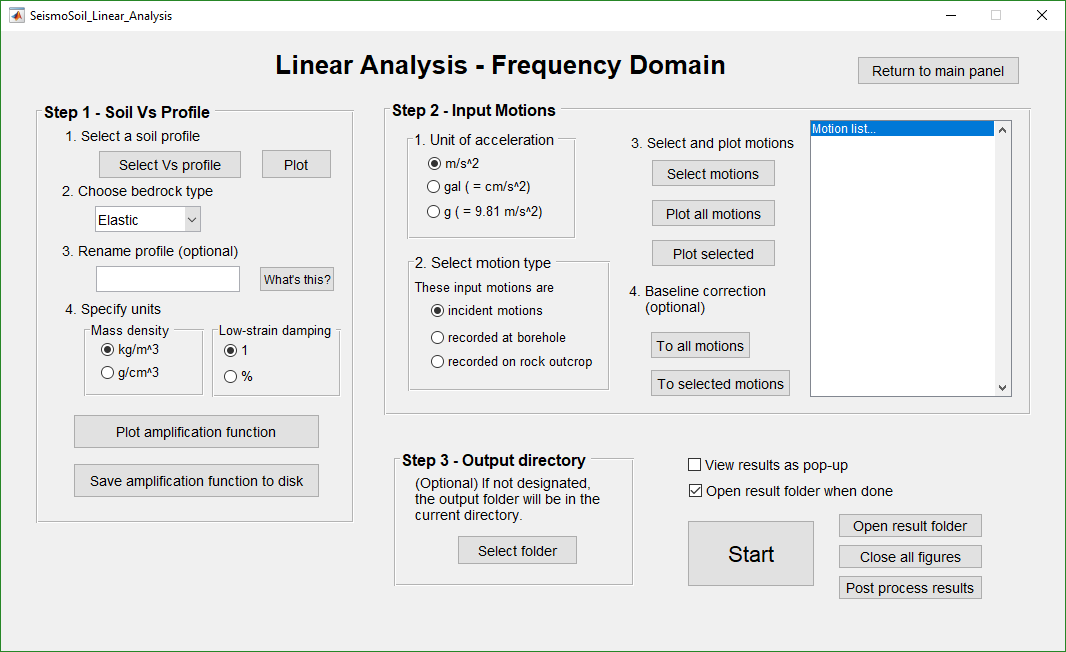
\includegraphics[width=0.99\textwidth]{linear_panel.png}\\
  %\caption{}\label{}
\end{figure}


Please note that in Step 1.2 and Step 3.2, bedrock type and motion type should be chosen. Careful consideration is strongly recommended here, since different combinations of these two can lead to rather different results.  Please refer to the notes in Section~\ref{sec:bedrock-type-and-motion-location} for a detailed explanation of how to make the choice.

The user interface for equivalent linear method is shown below. (Frequency-dependent equivalent linear method has identical interface.) Similarly to the linear analysis, the users can follow the procedures indicated on the panel and import the corresponding data.

\begin{figure}[H]
\centering
  % Requires \usepackage{graphicx}
  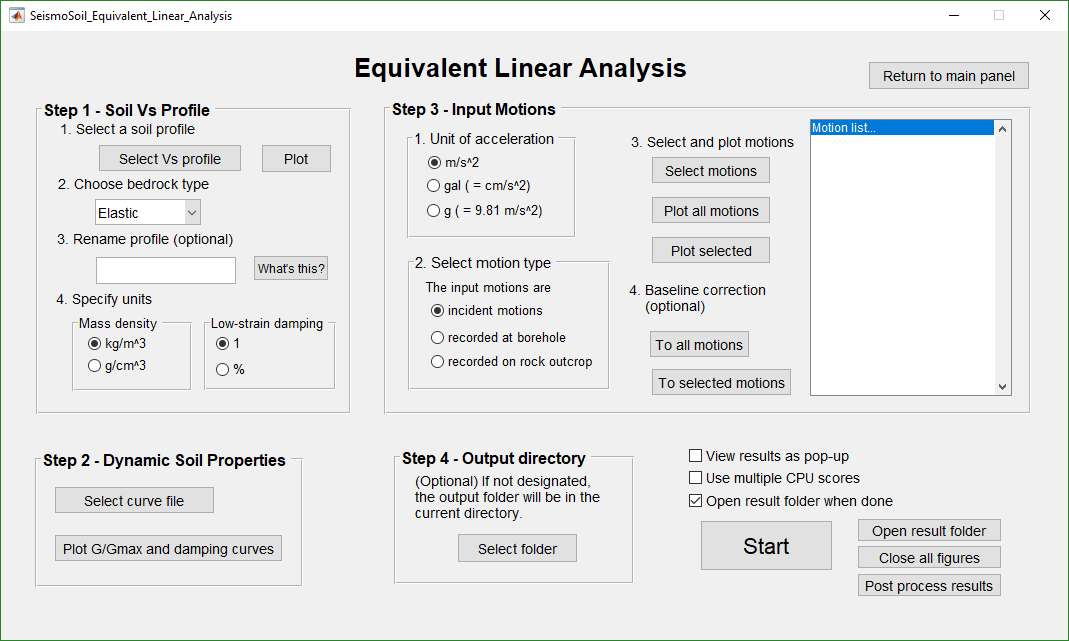
\includegraphics[width=0.99\textwidth]{equivalent_linear_panel.png}\\
  %\caption{}\label{}
\end{figure}

On the bottom-right corner of the panel, there are two check-box options. The second check box is self-explanatory, and the first check box controls whether figures of the simulation results will pop out. Note that the same figures will always be saved to the hard drive as PNG format.

\newpage
The user interface for \emph{HH} nonlinear analysis is shown below. The users should have no problem following the procedures indicated on the panel and import the corresponding data. 

The interface for \emph{H4} is the same as for \emph{HH}, and the interface for \emph{H2} nonlinear analysis differs slightly with \emph{HH} only in ``step 3'', where \emph{H2} only requires one input file, namely, \textsf{H2\_n.txt}.

\begin{figure}[H]
\centering
  % Requires \usepackage{graphicx}
  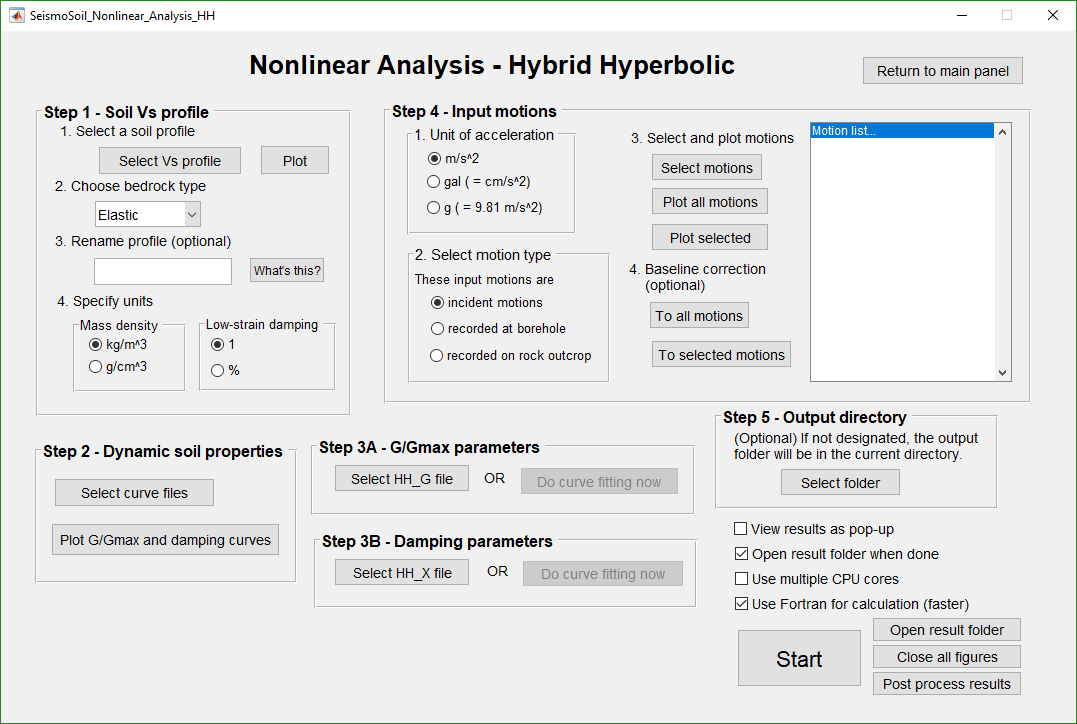
\includegraphics[width=0.99\textwidth]{HH_panel.png}\\
  %\caption{}\label{}
\end{figure}

\subsection{Notes on parallel computing}

Note that, on the bottom-right corner of the panel, there are two additional check boxes. ``Use multiple CPU cores'' controls whether or not SeismoSoil utilizes multiple cores of your CPU. If this box is checked, multiple ground motions will be processed in your CPU simultaneously, making the simulation approximately $n$ times faster, where $n$ is the total number of cores (not threads) of your CPU.

\subsection{Notes on Fortran kernel}

The box ``Use Fortran for calculation (faster)'' is checked by default. When checked, SeismoSoil calls the Fortran executables ({\textsf{TDLinear.exe}}, {\textsf{FDEQ.exe}}, {\textsf{NLH2.exe}}  {\textsf{NLH4.exe}}, {\textsf{NLEPP.exe}}, and \textsf{NLHH.exe}) to do the calculation, which is much faster than in MATLAB (the unchecked case). It is recommended that the user always check this box.

\newpage
\subsection{Notes on bedrock type and input motion location}\label{sec:bedrock-type-and-motion-location}

SeismoSoil has two options of bedrock in the numerical scheme: rigid and elastic. It also accepts three types of input motion: incident motion at the bedrock, total motion at the bedrock (or borehole recorded motion, or sometimes referred as the ``within motion''), and total motion on rock outcrop---as shown in the figure below. So there are six combinations:

\noindent\textbf{A)	Borehole recorded motion, with:}
\vspace{-10pt}
\begin{enumerate}
\item \textbf{Rigid bedrock} -- suitable when the borehole motion is known and prescribed (for example, you are using a KiK-net borehole recording as the input ground motion)
\item \textbf{Elastic bedrock} -- for this combination, the software generates a error message and does not do the simulation. Because elastic/viscoelastic bedrock means that the rock outcrop site has its own site response. The traditional approach of dividing the motion by 2 and using it as incident, or directly using the rock outcrop motion as total motion at the base of the profile are not correct and should be avoided if needed. The users are encouraged to remove this response by performing rock outcrop deconvolution to the incident motion, and then run the analysis with other appropriate motion-bedrock combinations.
\end{enumerate}

\begin{wrapfigure}{r}{0.45\textwidth}
\begin{center}
  % Requires \usepackage{graphicx}
  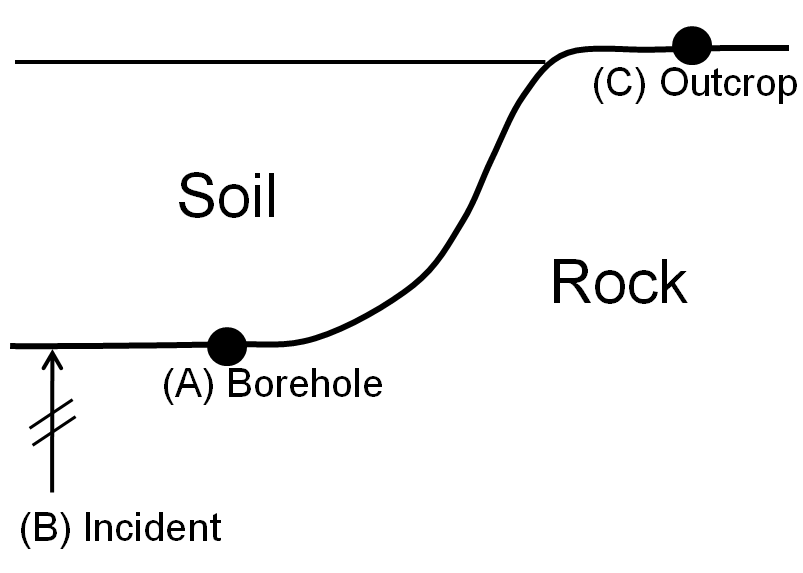
\includegraphics[width=0.45\textwidth]{three_motion_types.png}\\
  %\caption{}\label{}
\end{center}
\end{wrapfigure}

\noindent\textbf{B) Incident motion, with:}
\vspace{-10pt}
\begin{enumerate}
\item \textbf{Rigid bedrock} -- in this case, the borehole motion, i.e., the total motion, is equal to the outcrop motion, and twice the incident motion
\item \textbf{Elastic bedrock} -- in this case, the input motion is the borehole motion free of downgoing waves
\end{enumerate}

\noindent\textbf{C) Rock outcrop motion, with:}
\vspace{-10pt}
\begin{enumerate}
\item \textbf{Rigid bedrock} -- this combination is identical to combination A1
\item \textbf{Elastic bedrock} -- use with caution: the actual motion at the soil-rock interface is slightly different from the outcrop motion, so it is recommended that the users deconvolve the rock outcrop motion to incident motion, and use combination B2
\end{enumerate}

The choice of different combinations affects how SeismoSoil calculates the site response, and thus the results of simulations. Figure~\ref{fig:three-types-of-TF} on page \pageref{fig:three-types-of-TF} shows three different types of linear amplification factors corresponding to different choices of bedrock-motion combinations.


\newpage
\subsection{Output files}

The output data files include the following (assuming the input motion name is M1):

\begin{small}
\begin{itemize}
\item \textsf{M1\_accel\_on\_surface.txt} - Acceleration time history on ground surface. Two columns: time array (on the left) and acceleration (on the right).
\item \textsf{M1\_max\_a\_v\_d.txt} - Maximum acceleration, velocity, and displacement of each layer
\item \textsf{M1\_max\_gamma\_tau.txt} - Maximum strain and stress of each layer
\item \textsf{M1\_nonlinear\_TF\_raw.txt} - Nonlinear transfer function (absolute value, and unprocessed). Two columns: frequency array (on the left) and amplification factor (on the right)
\item \textsf{M1\_nonlinear\_TF\_smoothed.txt} - Nonlinear transfer function (absolute value, smoothed, using Konno-Ohmachi algorithm\footnote{Please refer to Section~\ref{sec:konno-ohmachi} on page \pageref{sec:konno-ohmachi} for details of the Konno-Ohmachi smoothing algorithm}). The format is the same as the raw transfer function.
\item \textsf{M1\_re-discretized\_profile.txt} - Re-discretized soil profile used internally in the simulation, usually finer than the original layering\footnote{Please refer to Section~\ref{sec:rediscretization} on page \pageref{sec:konno-ohmachi} for details of layer re-discretization.}
\item \textsf{M1\_time\_history\_accel.txt} - Acceleration time history of every layer. Each column represents the time history of one layer. And the columns from left to right represent the soil layers from the surface to the bedrock. The time array is not included.
\item \textsf{M1\_time\_history\_veloc.txt} - Velocity time history of every layer. Format same as above.
\item \textsf{M1\_time\_history\_displ.txt} - Displacement time history of every layer. Format same as above.
\item \textsf{M1\_time\_history\_strain.txt} - Strain time history of every layer. Format same as above.
\item \textsf{M1\_time\_history\_stress.txt} - Stress time history of every layer. Format same as above.
\end{itemize}
\end{small}

There are also three~\textsf{.png} figures corresponding to the data files.

\paragraph{Note on the units} The units in the output files \emph{\underline{are all SI units}} (sec, Hz, m, m/s, m/s/s, and Pa), and the unit of the output strains is 1 (not \%).

Along with the output text files, there are also three output figures generated for each analysis, as shown below:

\begin{figure}[H]
    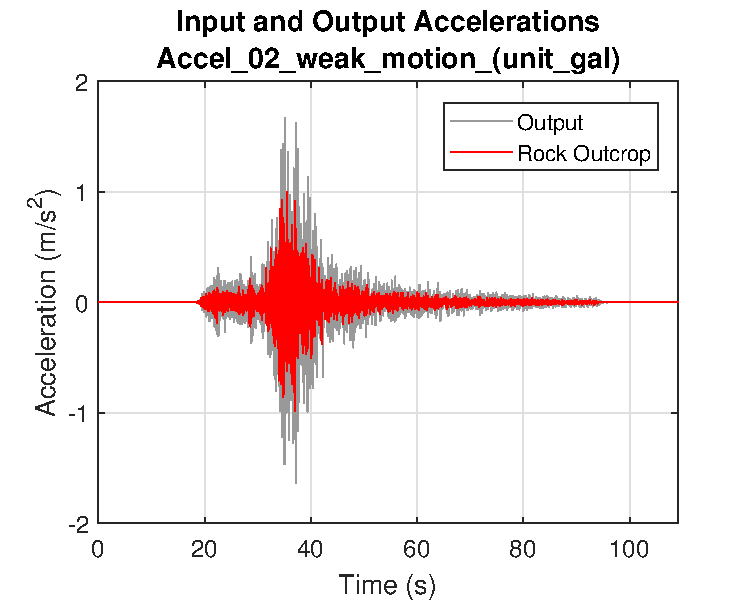
\includegraphics[width=0.47\textwidth]{Accel_02_weak_motion_(unit_gal)_accelerations.pdf}
    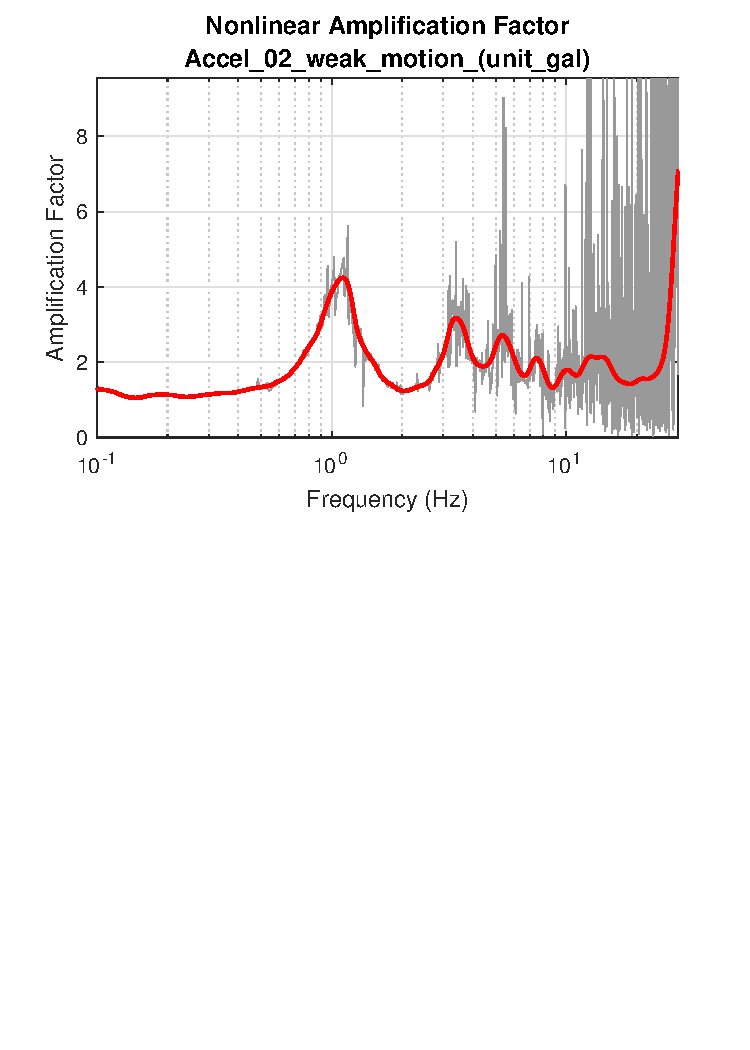
\includegraphics[width=0.52\textwidth]{Accel_02_weak_motion_(unit_gal)_nonlinear_TF.pdf}
\end{figure}

\begin{figure}[H]
    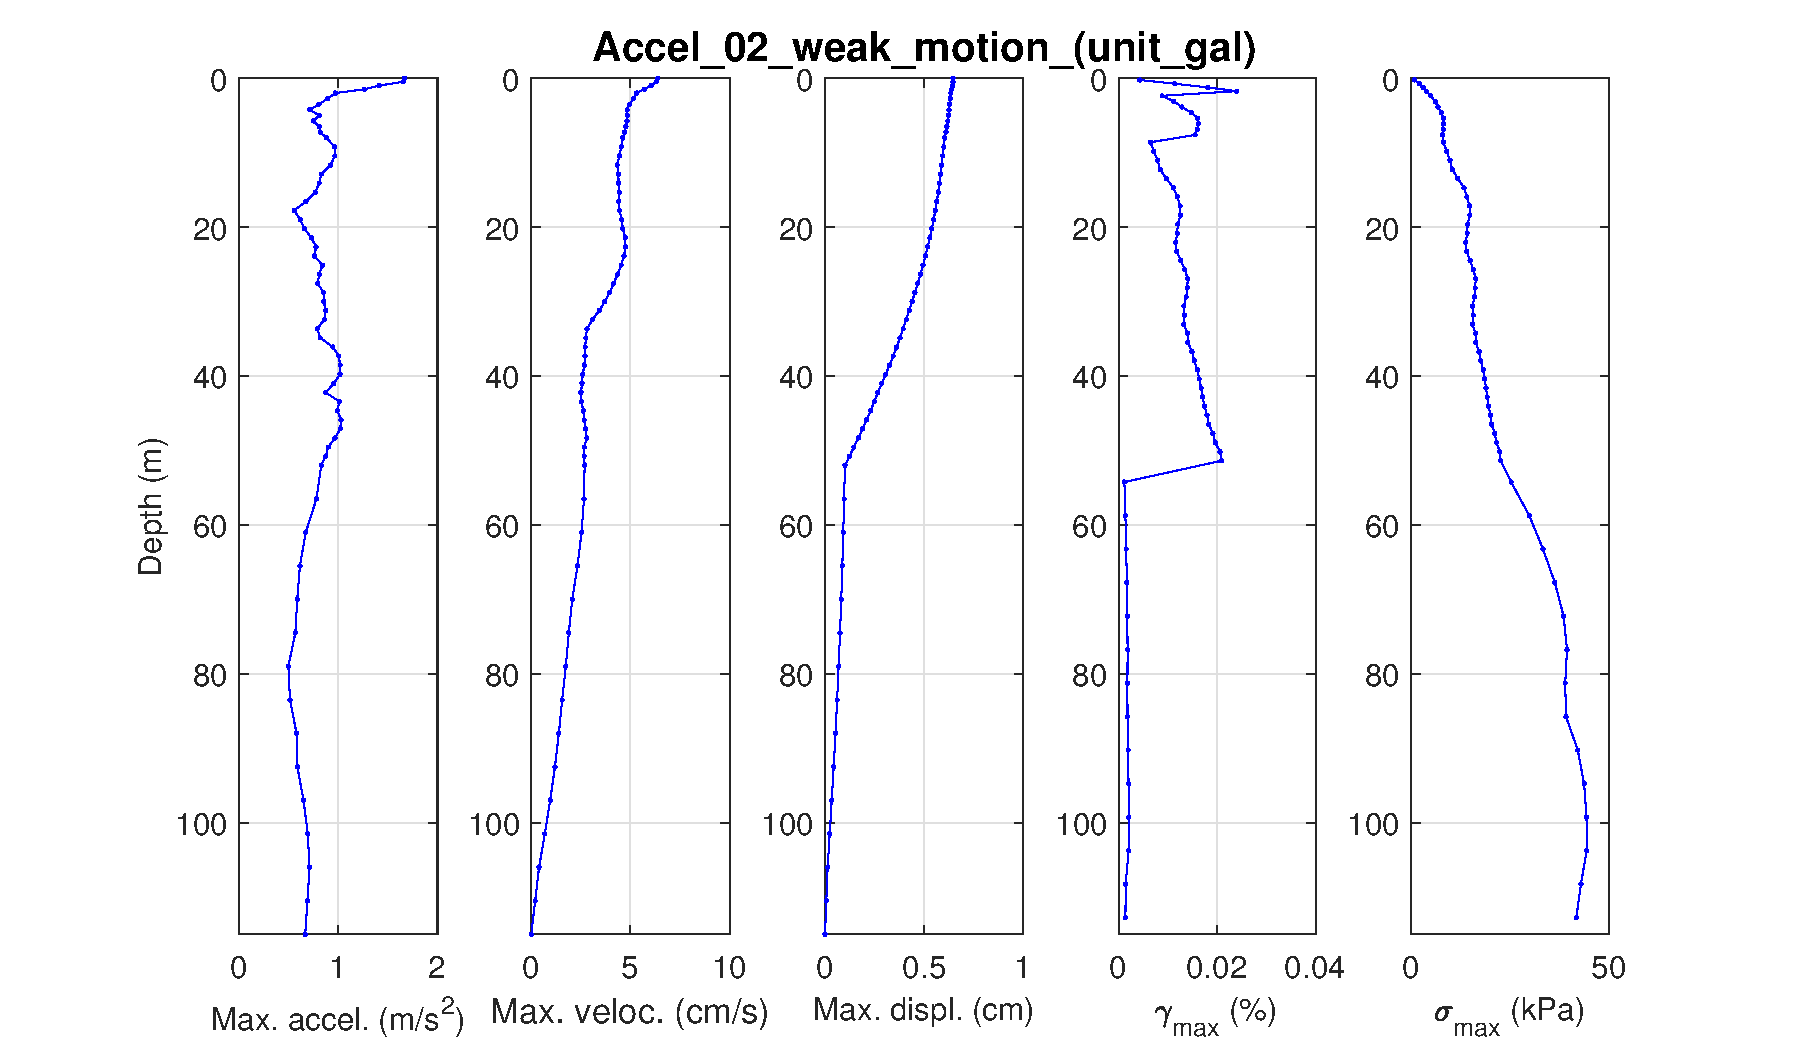
\includegraphics[width=\textwidth]{Accel_02_weak_motion_(unit_gal)_max_a_v_d_gamma_tau.pdf}
\end{figure}

\newpage
\subsection{Post processing tool}
A simple post processing panel is available, from clickng the ``\textsf{Post process results}'' results on the lower-right corner of any analysis panels (linear, equivalent linear, etc.). The \panel{post process results} panel is shown below.

\begin{figure}[H]
	\centering
	% Requires \usepackage{graphicx}
	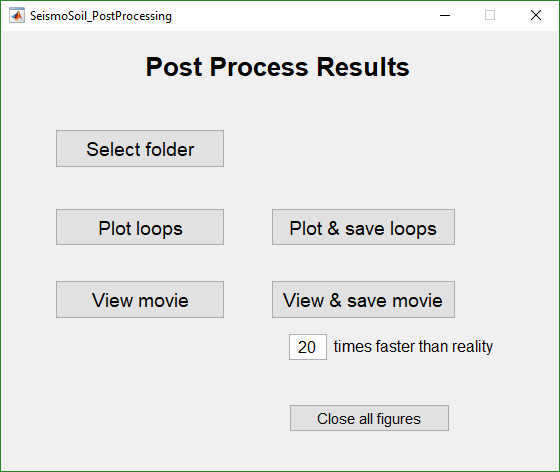
\includegraphics[width=0.50\textwidth]{PostProcessing.png}\\
\end{figure}

Click ``\textsf{Select folder}'', and choose a folder containing SeismoSoil output files. Click ``\textsf{Plot loops}'' to view the stress-strain loops of each layer (left). Click ``\textsf{View movie}'' to see animations of the ground deformation profile (right).

\begin{figure}[H]
	\centering
	\subfloat{
	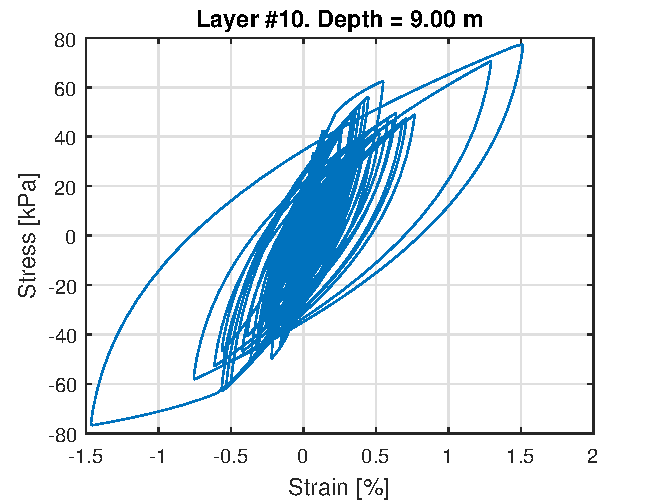
\includegraphics[width=0.49\textwidth]{stress_strain_loops.pdf}}
	\subfloat{
	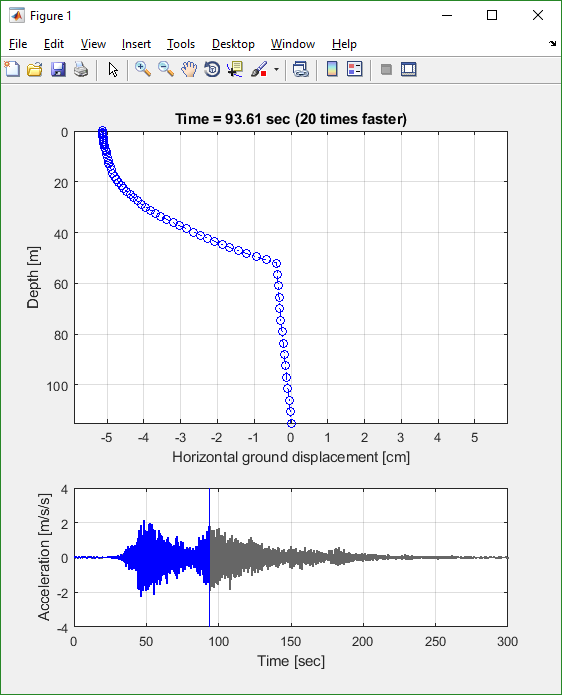
\includegraphics[width=0.42\textwidth]{view_movie.png}}
\end{figure}

\newpage
\section{Technical Manual}\label{sec:manual}

\subsection{Linear method}\label{sec:linear}

In linear approach, the soil is assumed as a Kelvin-Voigt solid, whose dynamic behavior is is described using a purely elastic spring and a purely viscous dashpot \citep{Kramer1996}, having two defining parameters, $G$ (soil modulus) and $\xi$ (soil damping ratio). Linear approach assumes $G$ and $\xi$ to remain unchanged in dynamic processes, which is not the case, especially when the ground motion intensity is strong.

In many cases, only the shear wave velocity ($V_S$) is known, but not the damping and density. Then the empirical rule proposed at the end of \ref{sec:soil_profile} can be used to calculate damping and density from $V_S$.

\subsubsection{Frequency domain linear method}

In frequency domain linear analysis, the amplification of ground motions by the soil layers are computed via transfer functions, using the following formula,
\begin{equation}\label{eq:freq-domain-amplification}
    a_{\text{out}}\left(t\right)=\text{IFT}\left[H\left(\omega\right)\cdot\text{FT}\left[a_{\text{in}}(t)\right]\right]
\end{equation}
where $a_{\text{in}}(t)$ and $a_{\text{out}}$ are the input and output ground motions in time domain, FT[ ] and IFT[ ] represent Fourier transform and inverse Fourier transform, and $H(\omega)$ is the complex-valued transfer function in frequency domain, which can be solely determined by the soil property profile.

The following paragraphs show the derivation of $H(\omega)$ from the soil properties.

Let $ j $ denote the soil layer index, and $ A_j $ and $ B_j $ the upgoing and downgoing SH wave displacement amplitudes at the $ j $-th layer.  In this case, the following relationship holds for every $ j $:
\begin{equation}
 \left\{\begin{array}{c}
A_{j+1} \\
B_{j+1}
\end{array} \right\} = \left[\begin{array}{cc}
\f{1}{2}(1+\alpha^*_j)\mrm{e}^{ik^*_jh_j} & \f{1}{2}(1-\alpha^*_j)\mrm{e}^{-ik^*_jh_j} \\
\f{1}{2}(1-\alpha^*_j)\mrm{e}^{ik^*_jh_j} & \f{1}{2}(1+\alpha^*_j)\mrm{e}^{-ik^*_jh_j}
\end{array} \right]\cdot \left\{\begin{array}{c}
A_j \\
B_j
\end{array} \right\}  \eqdef \mathbf{D}_j\cdot \left\{\begin{array}{c}
A_j \\
B_j
\end{array} \right\}
\end{equation}
where $ \alpha_j^* = \displaystyle\f{\rho_j V^*_{S,j}}{\rho_{j+1} V^*_{S,j+1}}$ is the complex impedance ratio of two successive layers $ j $ and $ (j+1) $;  \newline $ V^*_{S,j} = V_{S,j}\cdot\sqrt{1+2i\xi_j}$ is the complex shear wave velocity of layer $ j $; $ h_j $ is the thickness of layer $ j $; and $ k^*_j = \displaystyle\f{\omega}{V^*_{S,j}} = \f{k_j}{1+i\xi_j}$ is the complex wave number of layer $ j $, where $ \omega $ is the angular frequency.

Hence
\begin{equation}
	\left\{\begin{array}{c}
A_j \\
B_j
\end{array} \right\} = \mathbf{D}_{j-1} \left\{\begin{array}{c}
A_{j-1} \\
B_{j-1}
\end{array} \right\} = \mathbf{D}_{j-1}\mathbf{D}_{m-2}\left\{\begin{array}{c}
A_{j-2} \\
B_{j-2}
\end{array} \right\} = \cdots = \mathbf{D}_{j-1}\mathbf{D}_{j-2}\cdots\mathbf{D}_{1}\left\{\begin{array}{c}
A_{1} \\
B_{1}
\end{array} \right\}
\label{eq:j_to_1}
\end{equation}
where $ A_1 = B_1 = S/2 $, and $ S $ is the total surface displacement amplitude.

Let $ \mathbf{E}_{j-1} = \mathbf{D}_{j-1}\mathbf{D}_{j-2}\cdots\mathbf{D}_{1} $, thus Equation~\eqref{eq:j_to_1} becomes
\begin{equation}\label{eq:j-to-1b}
\left\{\begin{array}{c}
A_j \\
B_j
\end{array} \right\} = \mathbf{E}_{j-1}\left\{\begin{array}{c}
A_1 \\
B_1
\end{array} \right\}  = \left[\begin{array}{cc}
E_{j-1}^{\langle 11\rangle} & E_{j-1}^{\langle 12\rangle} \\
E_{j-1}^{\langle 21\rangle} & E_{j-1}^{\langle 22\rangle}
\end{array} \right]\left\{\begin{array}{c}
S/2\\
S/2
\end{array} \right\}
\end{equation}

Equation~\eqref{eq:j-to-1b} relates the displacement amplitudes at the top of the $j$-th layer to the layer on ground surface. Using this equation we can also relate the displacement amplitudes of any two layers, $j$ and $k$,
\begin{equation}
    \left\{\begin{array}{c}
    A_j \\
    B_j
    \end{array} \right\} = \mathbf{E}_{j-1}\cdot\mathbf{E}_{k-1}^{-1}\cdot\left\{\begin{array}{c}
    A_k \\
    B_k
    \end{array} \right\}
\end{equation}
And if $m$ is the total number of soil layers (excluding the underlying bedrock), the displacement amplitudes between the top of bedrock and the top of ground surface is
\begin{equation}\label{eq:m-to-1}
\left\{\begin{array}{c}
A_m \\
B_m
\end{array} \right\} = \mathbf{E}_{m-1}\left\{\begin{array}{c}
A_1 \\
B_1
\end{array} \right\}  = \left[\begin{array}{cc}
E_{m-1}^{\langle 11\rangle} & E_{m-1}^{\langle 12\rangle} \\
E_{m-1}^{\langle 21\rangle} & E_{m-1}^{\langle 22\rangle}
\end{array} \right]\left\{\begin{array}{c}
S/2\\
S/2
\end{array} \right\}
\end{equation}

Referring to Figure~\ref{fig:three-types-of-input-motions}, three types of transfer functions can be written,


\begin{figure}[h]
    \centering
  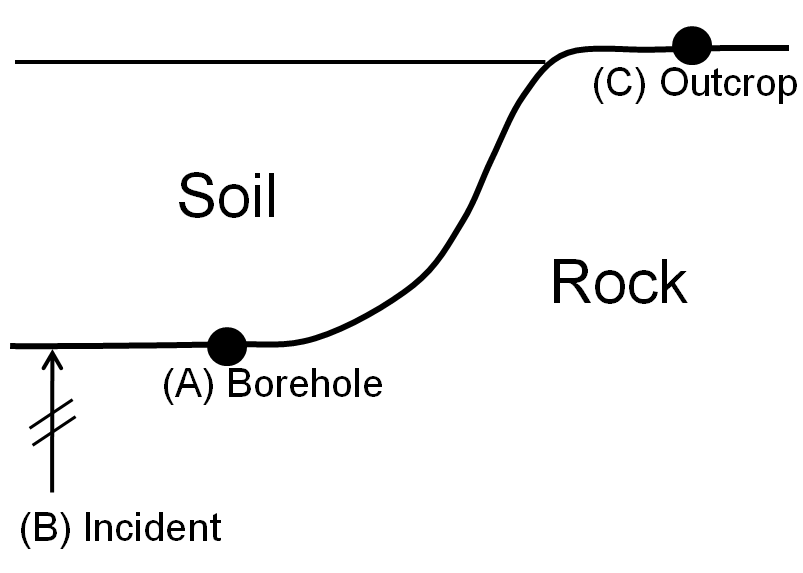
\includegraphics[width=0.45\textwidth]{three_motion_types.png}\\
  \caption{Three types of input motions}\label{fig:three-types-of-input-motions}
\end{figure}

\textsf{(A)} The ``surface to borehole'' (surface motion to total borehole motion) transfer function:
\begin{equation}
H_{\text{A}}(\omega)  = \displaystyle\frac{\text{Ampl}(u_1)}{\text{Ampl}(u_{m-\text{(total)}})} = \frac{S/2 + S/2}{A_m+B_m} = \frac{2}{E_{m-1}^{\la 11\ra} + E_{m-1}^{\la 12\ra}+E_{m-1}^{\la 21\ra} + E_{m-1}^{\la 22\ra}}
\end{equation}
%and the absolute value of $H_{\text{A}}(\omega)$ is the amplification factor
%\begin{equation}
%\mathrm{AF}_{\txt{S-BH}}(\omega) = |\mathrm{TF}_{\txt{S-BH}}(\omega)| = \f{2}{\left|E_{N-1}^{\la 11\ra} + E_{N-1}^{\la 12\ra}+E_{N-1}^{\la 21\ra} + E_{N-1}^{\la 22\ra}\right|}
%\end{equation}

\textsf{(B)} The ``surface to incident'' (surface motion to incident motion at borehole) transfer function is
\begin{equation}
H_{\text{B}}(\omega) = \f{S/2+S/2}{A_m} =\f{2}{E_{m-1}^{\la 11\ra} + E_{m-1}^{\la 12\ra}}
\end{equation}

\textsf{(C)} The ``surface to rock outcrop'' (motion at soil surface to motion at rock outcrop site's surface) transfer function is
\begin{equation}
H_{\text{C}}(\omega) = \f{S/2+S/2}{2A_m} = \f{1}{E_{m-1}^{\la 11\ra} + E_{m-1}^{\la 12\ra}}
\end{equation}

The three types of amplification functions of a same site, plotted together on the same graph, are shown in Figure~\ref{fig:three-types-of-TF}.

\begin{figure}[h]
    \centering
  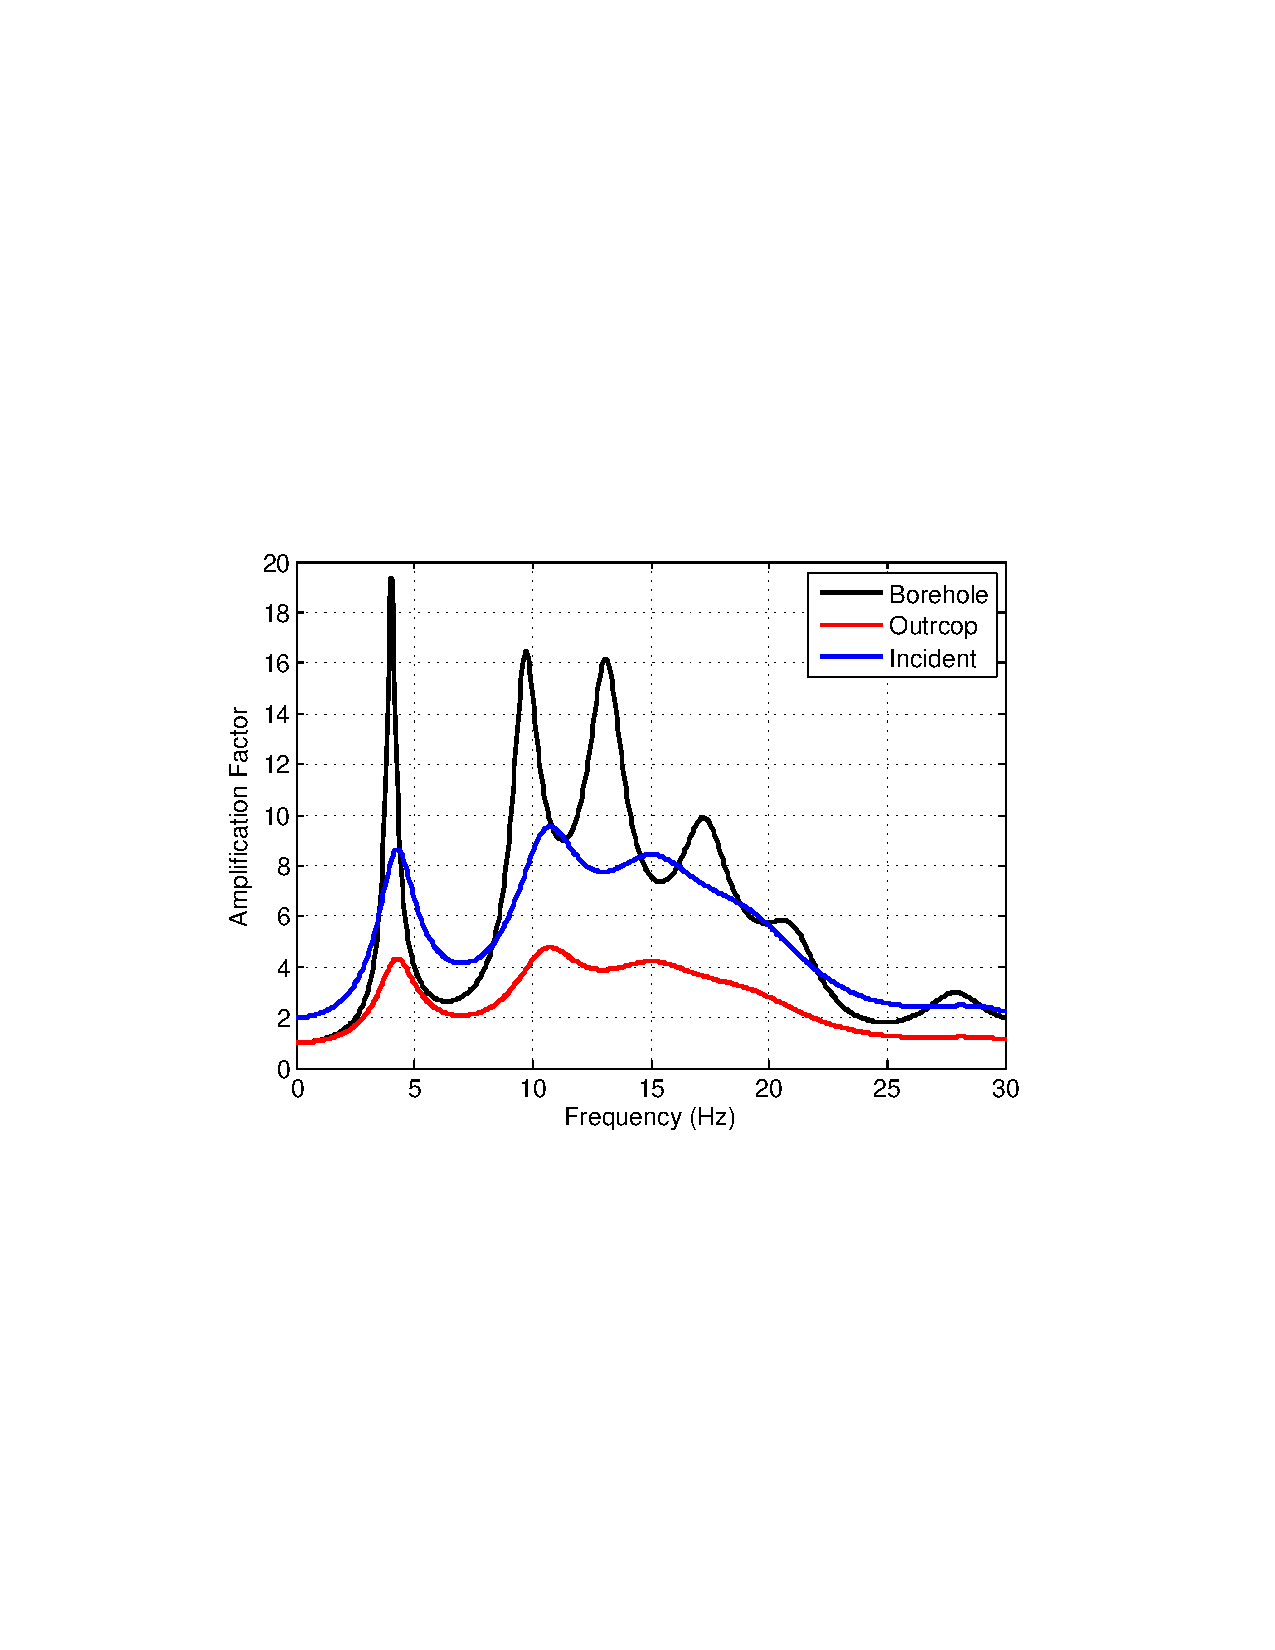
\includegraphics[width=0.6\textwidth]{three_types_of_TF.pdf}\\
  \caption{Three types of linear transfer functions}\label{fig:three-types-of-TF}
\end{figure}




\subsubsection{Time domain linear method}

The time domain linear approach solves the wave propagation functions directly in the time domain, using the finite difference scheme. The soil properties remain unchanged during the entire duration of shaking. In order to incorporate $G$ and $\xi$ information from the input into the time domain scheme, a numerical model aiming at approximating the frequency independent damping behavior of soil is used. The degree of approximation is satisfactory, however not perfect. Therefore there is a slight difference between the result of frequency domain linear approach and time domain linear approach.

The merit of time domain linear approach is that it prevents the ``wrap-around'' phenomenon that frequency-domain linear approach sometimes has. Because of the underlying assumption of Fourier transform, that the signal in time domain being transformed ``starts from the beginning of time and lasts forever'', the response that corresponds to the end of the input ground motion appears at the beginning part of the output ground motion, i.e., ``wrapped-around''.  This phenomenon is especially pronounced when the input ground motion is synthetic and short, e.g., a Ricker wavelet.

For more details concerning how the temporal-spatial finite difference is carried out, please refer to Section~\ref{sec:nonlinear} on page \pageref{sec:nonlinear}.


\subsection{Equivalent linear method}\label{sec:equivalent-linear}

\subsubsection{Original equivalent linear method}

The equivalent linear approach, originally proposed by Harry Bolton Seed and Izzat M.~Idriss in 1970, and first programmed in SHAKE \citep{Schnabel1972SHAKE,shake91_manual}, is a modified linear approach which partly incorporates the nonlinear properties of soil. This approach accepts that modulus and damping of soil in a dynamic process are no longer the same as their initial values, which are $G_{\text{max}}$ and $\xi_{\text{small strain}}$. In order to determine the appropriate values for $G$ and $\xi$, the equivalent linear approach calculates linear site response (in frequency domain) once, obtaining the strain time histories at the center of each soil layer. Then, an ``effective'' strain value is picked for each layer, which is subsequently used to obtain an updated $G$ value and an updated $\xi$ value from the modulus reduction and damping curves. Linear site response is carried out once more, obtaining updated strain time histories and effective strains, which are used to update $G$ and $\xi$ again.  This process is repeated until convergence. The ground response after convergence is the result of the equivalent linear approach.

The detailed procedure of the equivalent linear approach in SeismoSoil is as follows.
\begin{enumerate}
    \item Re-discretize the existing soil layers based on shear wave velocities of each layer (for details, see Section~\ref{sec:rediscretization} on page \pageref{sec:rediscretization})
    \item Calculate linear transfer functions between each intermediate layer and the input point (can either be ``borehole'', or ``incident'', or ``outcrop'')
    \item Use Equation~\eqref{eq:freq-domain-amplification} to calculate acceleration time histories on the top of each soil layer
    \item Integrate acceleration time histories twice to get displacement time histories
    \item Use the displacements between two neighboring layers to calculate the approximate strain time histories at the mid-point of each layer
    \item Pick 65\% of the maximum absolute strain as the ``effective'' strain (for every layer)
    \item Pick updated $G$ and $\xi$ values according to the ``effective'' strains of each layer
    \item Check if the relative differences between two successive $G$ and $\xi$ values fall below 7.5\% (for every layer)
    \item If true, end the iteration; of not, repeat steps 2--8
    \item After 10 iterations, break out of the loop, regardless of convergence
\end{enumerate}

The equivalent linear approach does not reflect the real-world soil behavior in that it assumes constant $G$ and $\xi$ values for each layer, during the entire duration of the dynamic response. In fact, modulus and damping of soil change instantaneously with the strain level that the soil has. Also, different frequency components in the input motion are associated with different strain levels, thus increasing damping values indiscriminatively causes the high frequency components in a ground motions, which are usually not as intense as the low frequency ones, to attenuate excessively. This is especially obvious for deep and soft sites.

An example of linear, equivalent linear and true amplification factors is shown in Figure~\ref{fig:af_comparison}. The true amplifications factor is calculated from actual surface and borehole seismographs. From the figure, we can see that how much equivalent linear approach overdamps the high frequency components, and how linear approach might overestimate ground response at some particular frequencies.

\begin{figure}[h]
    \centering
  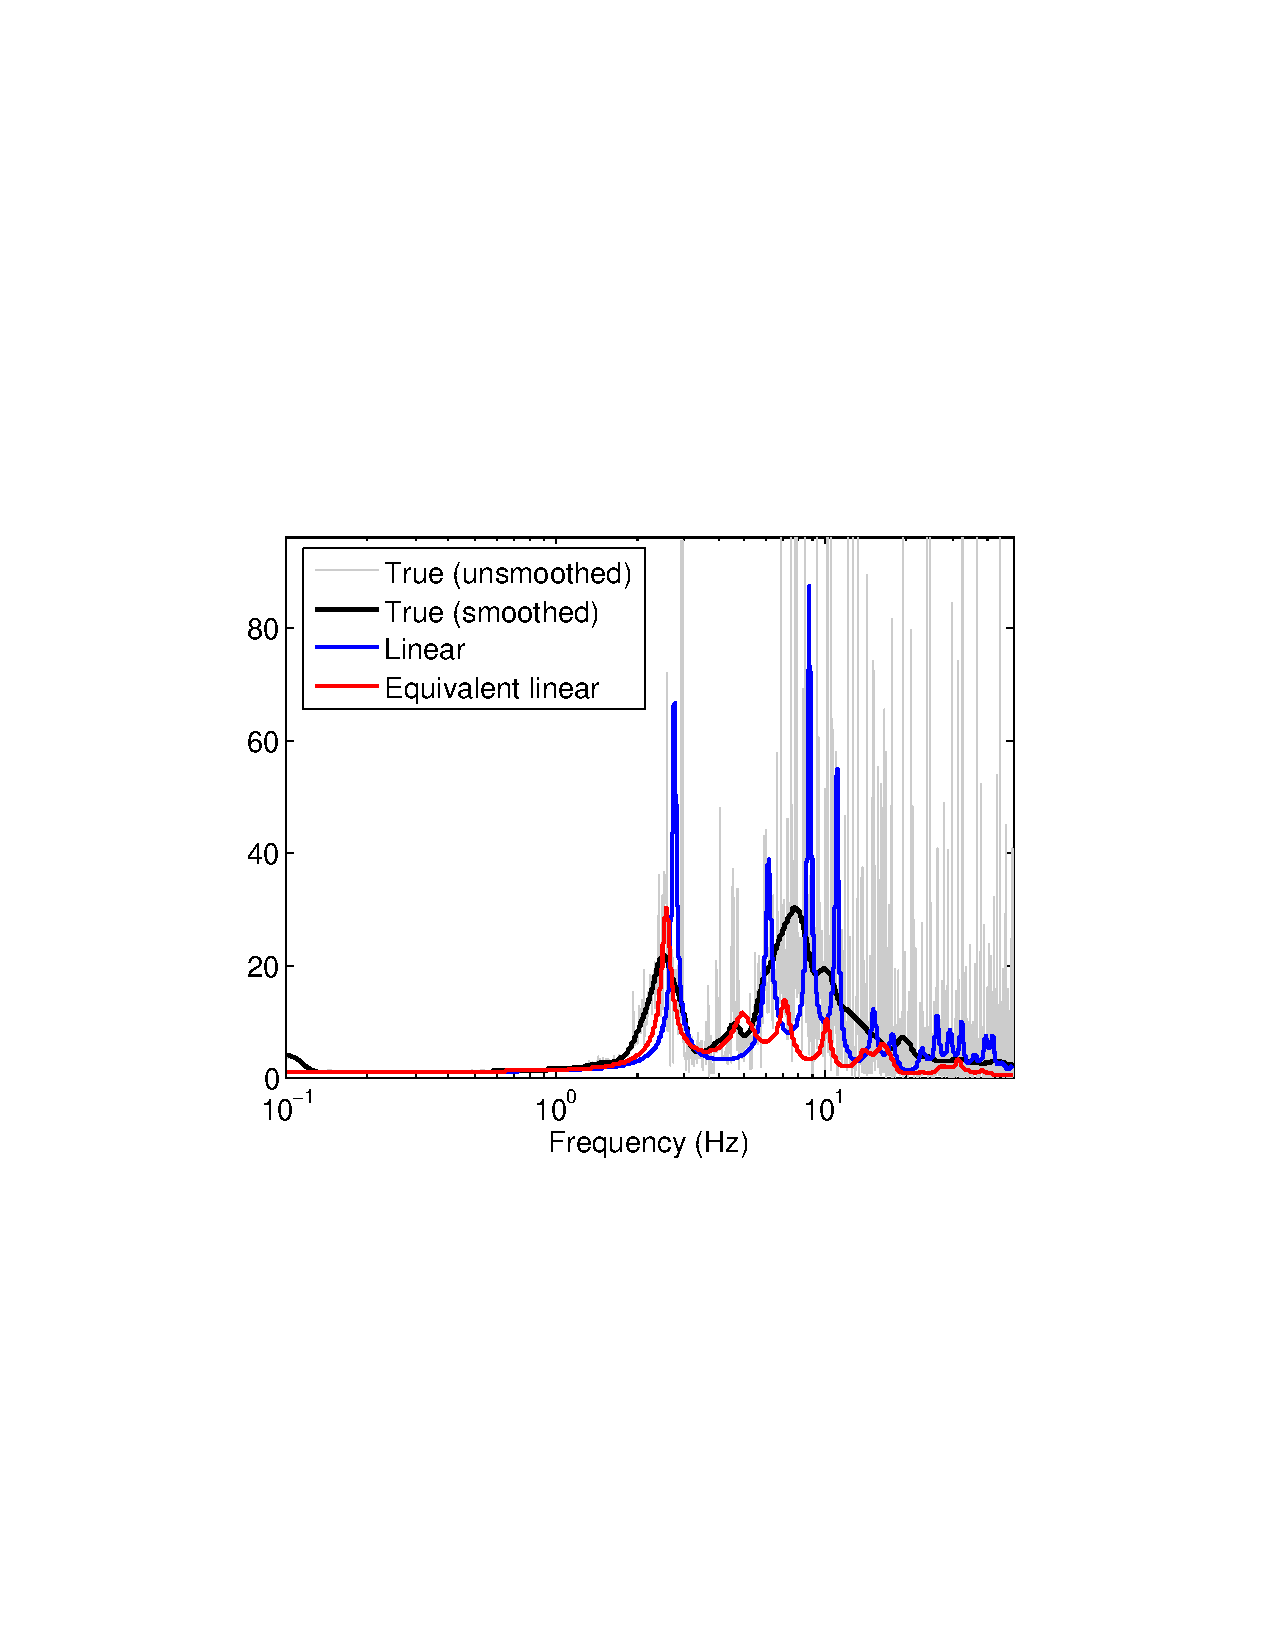
\includegraphics[width=0.5\textwidth]{amplification_factor_comparison.pdf}\\
  \caption{Comparison of amplifications factors. The ``true'' amplification factor is calculated from actual recordings.}\label{fig:af_comparison}
\end{figure}




\subsubsection{Equivalent linear method with frequency dependent modulus and damping}

The most obvious disadvantage of the original equivalent linear method is that it artificially suppresses higher frequencies, i.e., the higher frequency components in the simulated ground motion is unrealistically low compared to true outputs. \cite{Assimaki_Kausel_2002} proposed a frequency- and pressure-dependent equivalent linear method, which significantly improved the predictions of higher frequency contents. For the technical details of this method, please refer to the original paper

The kernel of this method within SeismoSoil is written in Fortran by Fabian Bonilla, for which the authors are very grateful.

\subsection{Nonlinear method}\label{sec:nonlinear}

The nonlinear analysis is performed in the time domain, using finite difference method (FDM). The features of the nonlinear method in SeismoSoil are
\begin{itemize}
	\item A memory-variable technique proposed by \cite{LiuPC_Archuleta_2006} to model small-strain damping is used, which, compared to Rayleigh and Caughey damping (both are frequency dependent), better simulates the frequency-independent small-stain damping in reality;
	
	\item The hysteresis (i.e., unloading/reloading) behavior model, proposed by \cite{Li_Assimaki_2010_BSSA}, based on the original model by \cite{Muravskii_2005}, is capable of simultaneously matching $G/G_{\max}$ and damping curves, yielding narrower and more realistic hysteresis loops than the loops by Masing rules.
	
	\item The stress-strain and damping behaviors of the soils are described by either the modified hyperbolic (MKZ) model \citep{Matasovic_Vucetic_1993}, or the hybrid hyperbolic (HH) model \citep{Shi_Asimaki_2017}. \footnote{The elasto-perfectly plastic model in SeismoSoil is only for demonstration purposes, and should not be used in practice due to its poor prediction accuracy.}
\end{itemize}

\subsection{The hybrid hyperbolic (HH) stress-strain model}\label{sec:HH_model}

The hybrid hyperbolic (HH) model is a new 1D stress-strain model proposed by \cite{Shi_Asimaki_2017}. This model can capture both small-strain soil behaviors (i.e., soil stiffness) and large-strain soil behaviors (i.e., shear strength), which is a step up from the currently popular MKZ model (proposed by \citealp{Matasovic_Vucetic_1993}) that only captures soil stiffness.

The nine parameters of the HH model all have clear physical meanings, which makes the HH model easy to calibrate using laboratory data. Also, when only the shear-wave ($V_S$) velocity profile is available at a site, the HH model parameters can also be calibrated using the empirical correlations listed in the Appendix of \cite{Shi_Asimaki_2017}.

The HH model can be used in the equivalent linear method as well as the nonlinear method. The benchmarking study in \cite{Shi_Asimaki_2017} has showed that the HH model significantly outperformed the MKZ model for both the equivalent linear and nonlinear methods.

Two examples of very strong motions (the 2011 $M_w$ 9.0 Tohoku Earthquake and 2003 $M_w$ 8.3 Hokkaido Earthquake) are shown below in Figure~\ref{fig:2003_and_2011_events}.

\begin{figure}[H]
    \noindent \begin{centering}
        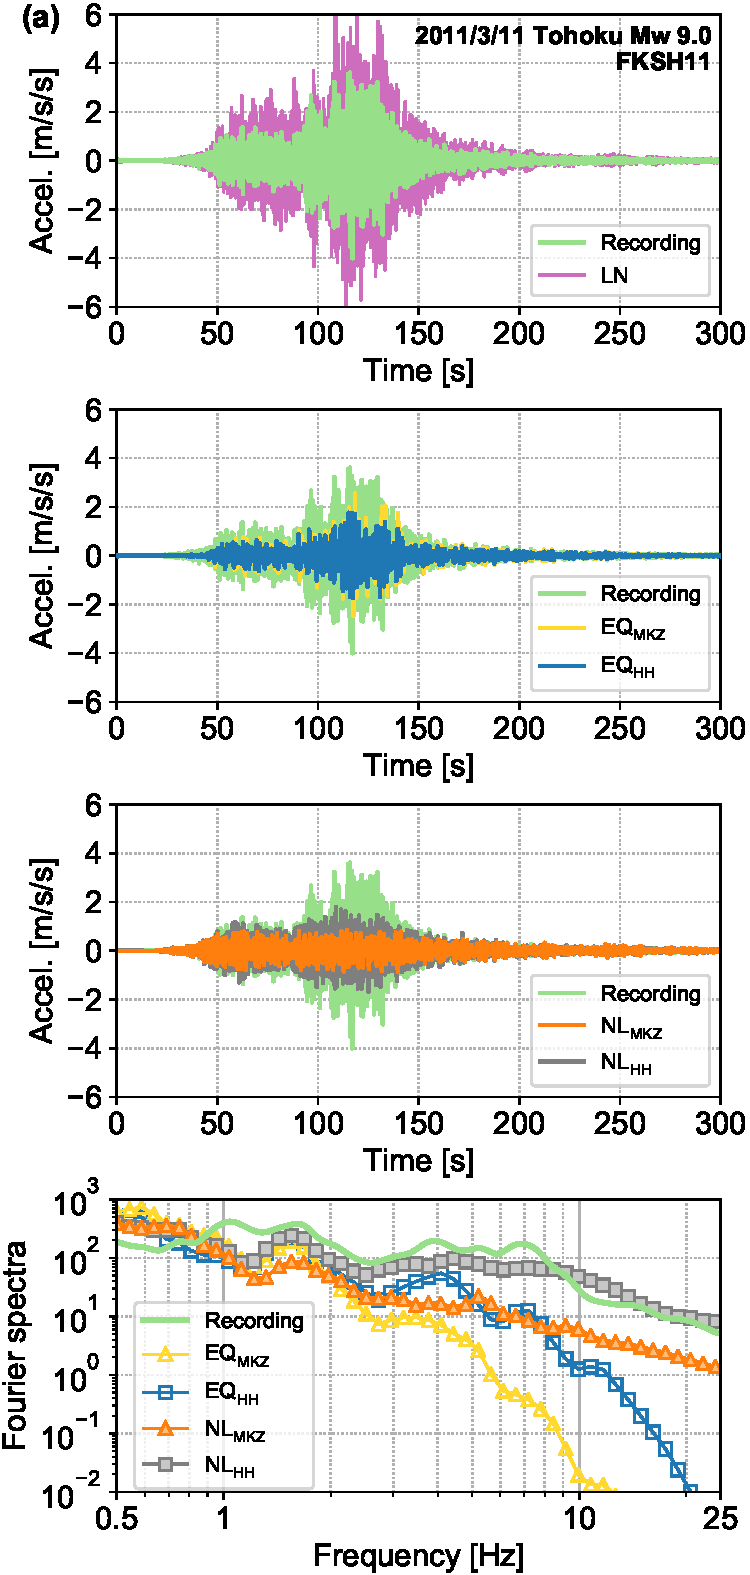
\includegraphics[width=0.47\textwidth]{Figure_15a_Tohoku_mainshock_FKSH11__a415}%~~~~~~~~~~
        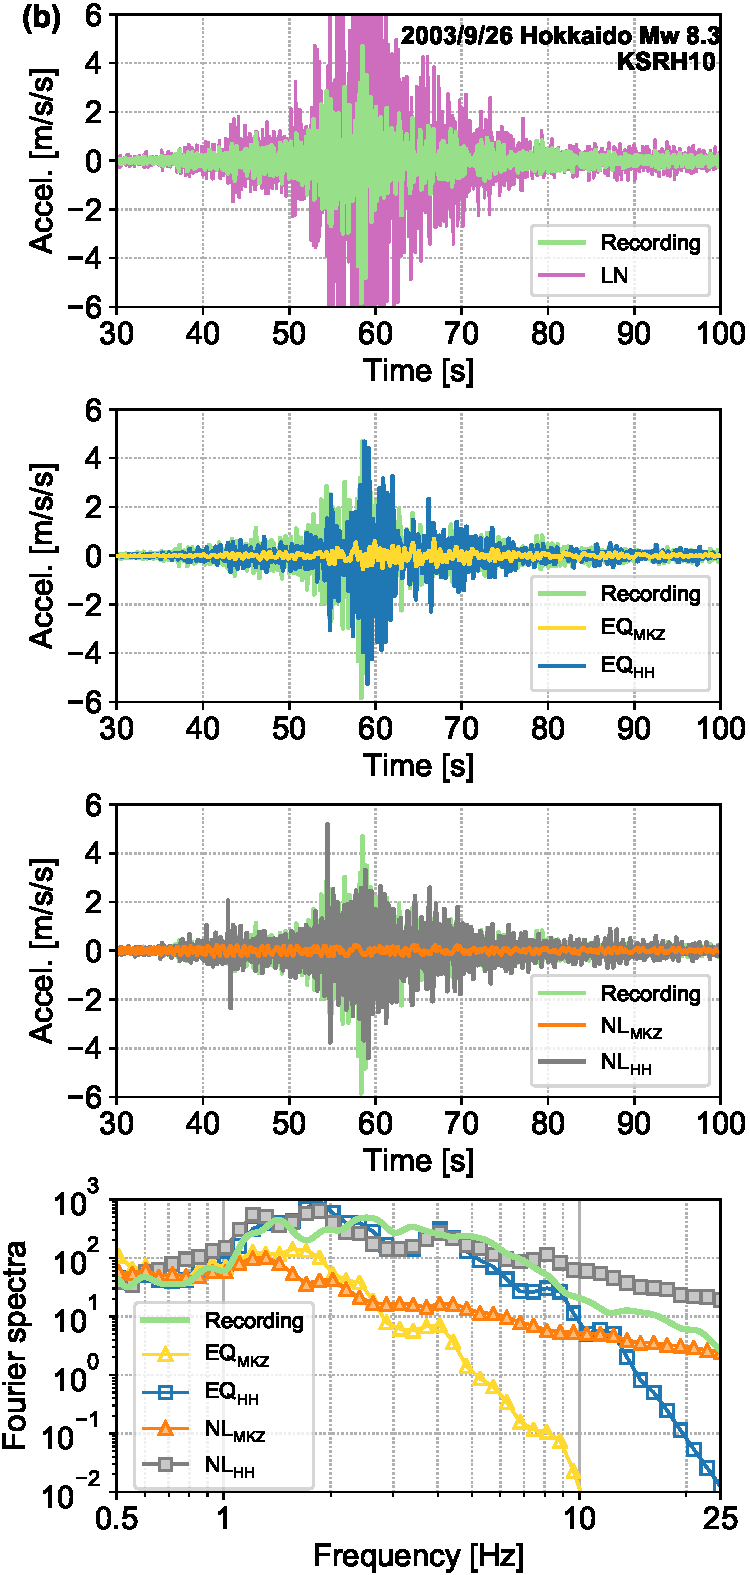
\includegraphics[width=0.47\textwidth]{Figure_15b_Hokkaido_mainshock_KSRH10__a415}
        \par\end{centering}
    
    \caption{Time history and Fourier spectra (smoothed) for the (a) 2011/3/11 $M_{\rm{w}}$~9.0 Tohoku Earthquake recorded at FKSH11 and (b) 2003/9/26 $M_{\rm{w}}$~8.3 Hokkaido Earthquake recorded at KSRH10. Recording and simulations are plotted together for comparison. (Figure adapted from \citealp{Shi_Asimaki_2017})}
    \label{fig:2003_and_2011_events}
\end{figure}

From Figure~\ref{fig:2003_and_2011_events} we can see that, for both equivalent linear (EQ) and nonlinear (NL) methods, the use of HH model (i.e., $\mathrm{EQ}_{\mathrm{HH}}$ and $\mathrm{NL}_{\mathrm{HH}}$) resulted in better prediction accuracy than using MKZ ($\mathrm{EQ}_{\mathrm{MKZ}}$ and $\mathrm{NL}_{\mathrm{MKZ}}$). Namely, the MKZ model would severely under-predict ground motions for strong events, because it does not capture the shear strength of soils. And for strong events, soils deform so much that they often approach or reach their shear strength.

Figure~\ref{fig:MKZ_vs_HH_curves} below shows two comparisons MKZ versus HH stress-strain curves for two different soil layers. On the left is a shallow soil layer with low overburden stress, and on the right is a deep layer with high overburden stress. In both cases, HH can capture the shear strength of soils, while MKZ can not. And this is the reason for MKZ to under-predict strong ground motions.

\begin{figure}[H]
    \centering
    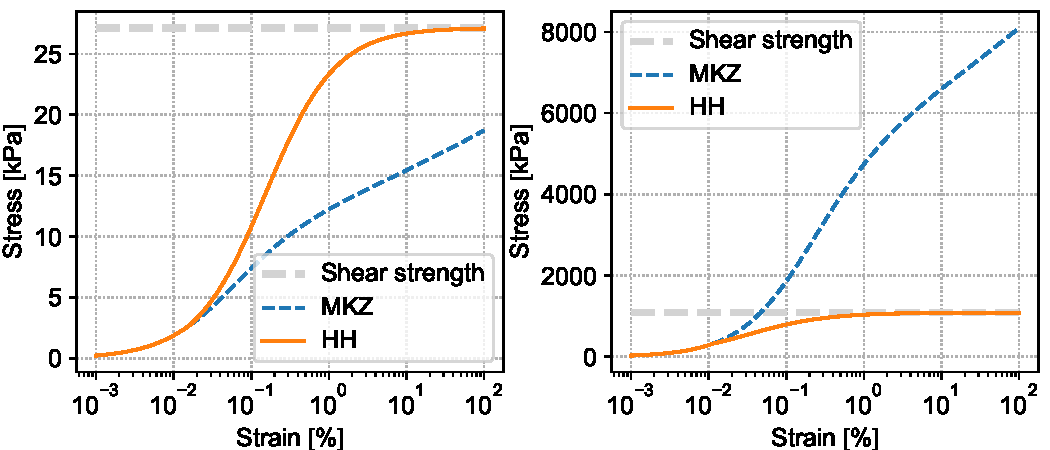
\includegraphics[width=0.76\textwidth]{MKZ_vs_HH_curves__a403.pdf}
    \caption{MKZ versus HH stress-strain curves.}
    \label{fig:MKZ_vs_HH_curves}
\end{figure}

Figure~\ref{fig:GoF_score_vs_max_strain} below shows the comprehensive goodness-of-fit scores of different site response analysis methods. The horizontal axis is the level of ground motions, and the vertical axis is the goodness-of-fit score (0 is perfect prediction, positive numbers are over-prediction, and negative numbers are under-prediction). And we can clearly see that equivalent linear or nonlinear methods that use the MKZ model under-predicts medium-to-strong ground motions, while simulations using the HH model provide quite satisfactory predictions.

\begin{figure}[H]
    \centering
    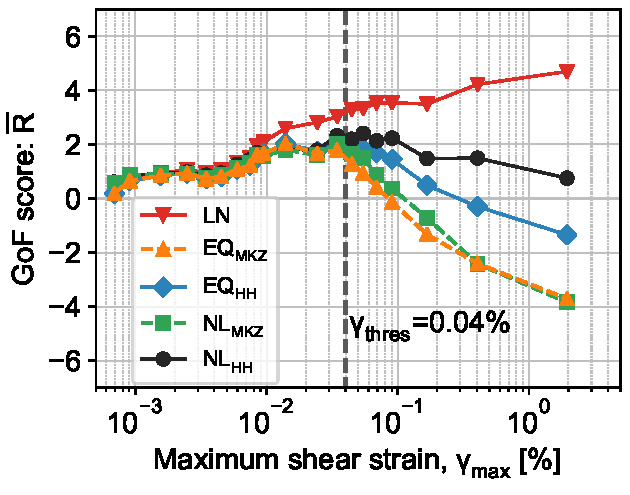
\includegraphics[width=0.48\textwidth]{Figure_14a_Average_GoF_score_vs_max_strain_9_stations_5_methods__a414a.pdf}
    \caption{MKZ versus HH stress-strain curves. (Adapted from \citealp{Shi_Asimaki_2017})}
    \label{fig:GoF_score_vs_max_strain}
\end{figure}


\newpage
\subsection{Miscellaneous technical details}

\subsubsection{Baseline correction}\label{sec:baseline-correction}

For various reasons, there are usually baseline offsets in the acceleration recordings, resulting in non-realistic shifts in the velocity and displacement time histories integrated from acceleration. To address this issue, we use high-pass filtering to remove the low frequency components in the acceleration recordings.

The procedures are as follows:
\begin{itemize}
	\item Remove ``pre-event'' mean value, which is defined as the average acceleration of the ``silent'' part 
	           of the recording, where the acceleration should be zero
	\item Cut off the beginning and end of the motion using the first zero-crossings as bounds
	\item Pad zeros at both ends of the acceleration array
	\item Apply zero-phase high-pass filtering (default cut-off frequency: 0.2~Hz; users can use other values)
	\item Adjust the filtered time series so that it is aligned chronologically with the original time series
\end{itemize}

The result of the baseline correction is shown in Figure~\ref{fig:baseline_result_duplicate}.% The advantage of the baseline correction in SeismoSoil is that the corrected signal is in sync with the uncorrected signal, and has the same number of data points.

\begin{figure}[H]
	\centering
	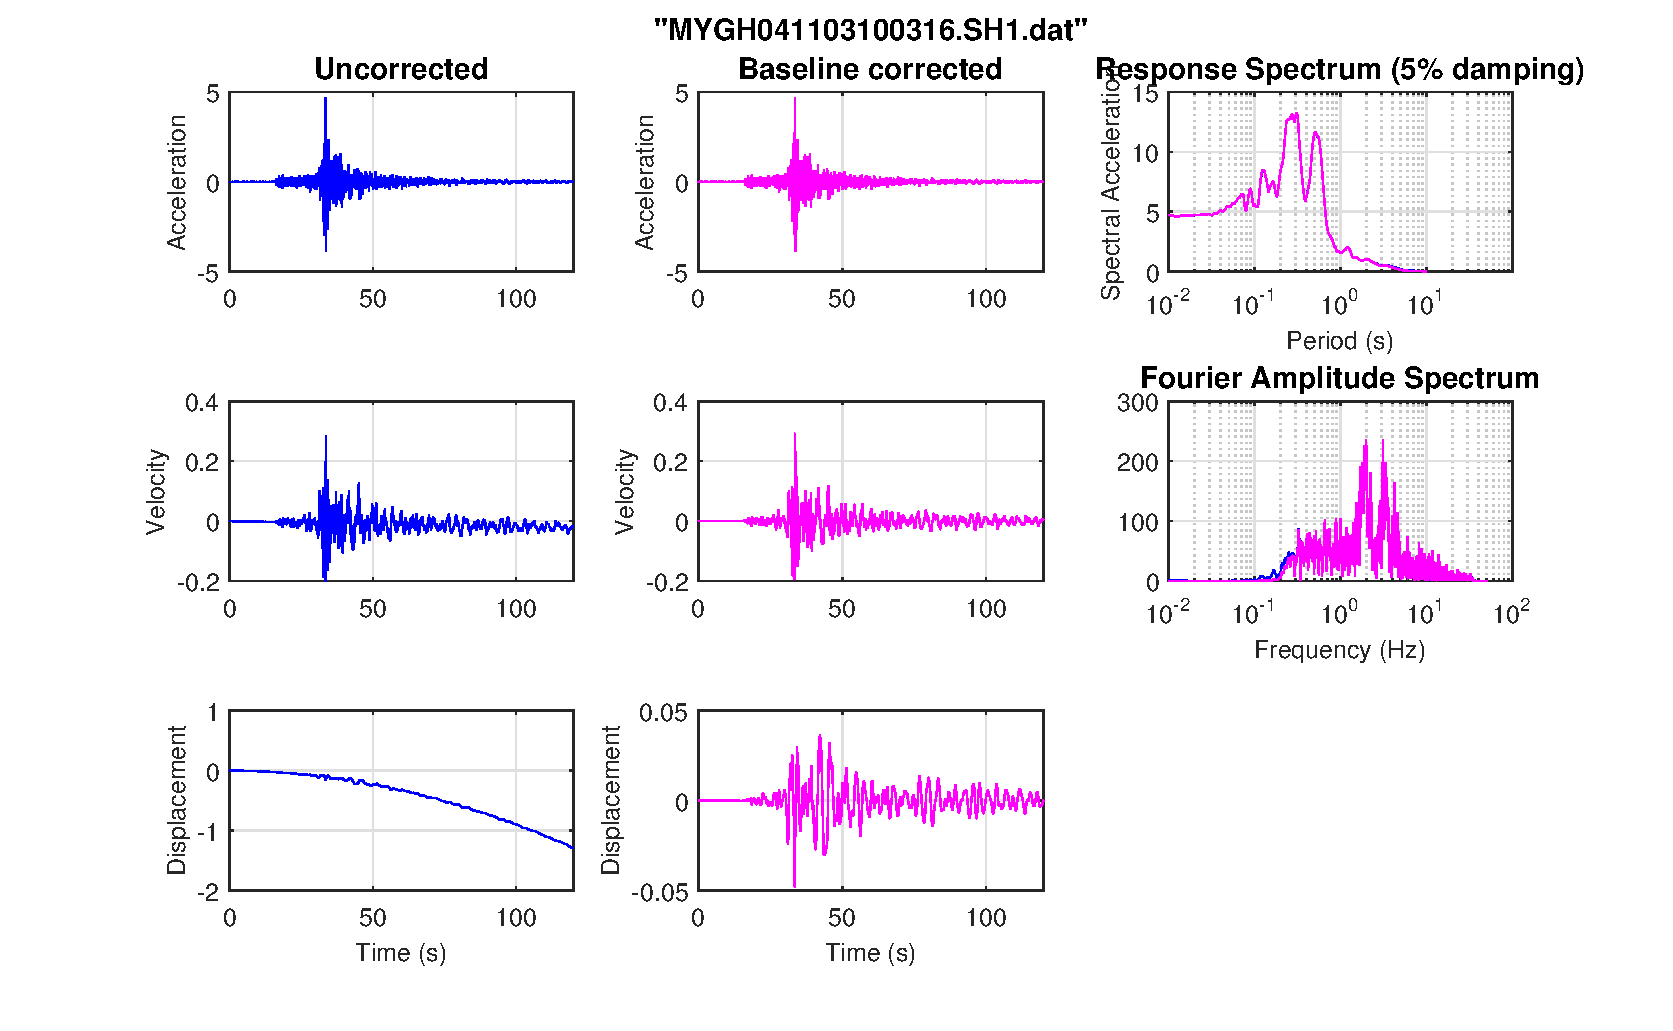
\includegraphics[width=.97\textwidth]{baseline_correction_result_new.pdf}\\
	\caption{Baseline correction result}
	\label{fig:baseline_result_duplicate}
\end{figure}

\subsubsection{Konno-Ohmachi smoothing of frequency spectra}\label{sec:konno-ohmachi}

Fourier spectra of a ground motion or spectral ratios (ratios of two Fourier spectra) usually have lots of spikes. A smoothing window applied to the spectral ratio is able to address this problem, making the spectra more easily understandable.

SeismoSoil uses two different kinds of spectral smoothing: uniform sine window and Konno-Ohmachi window in its Fourier spectra panel.

\begin{figure}[h]
	\centering
	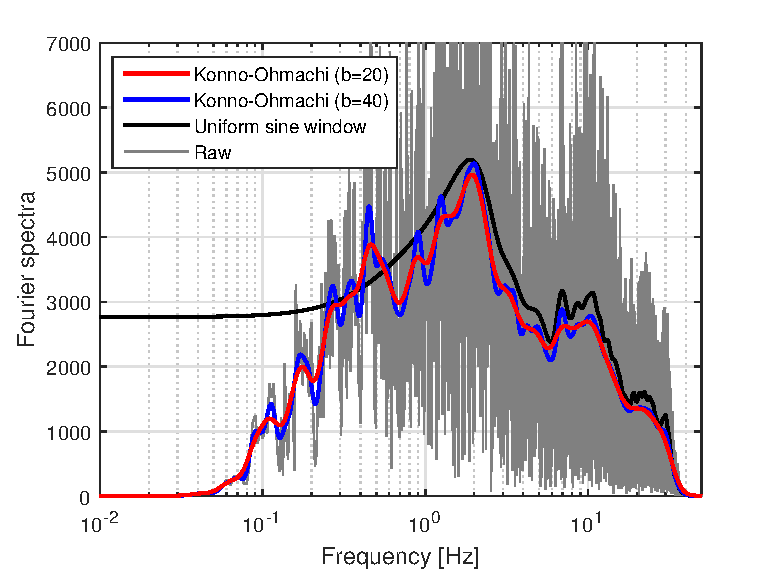
\includegraphics[width=0.65\textwidth]{different_smoothing_windows.pdf}
	\caption{Comparison of different smoothing windows}\label{fig:different_smoothing_windows}
\end{figure}

The most basic type of smoothing window is the uniform window, which means that the window width for different frequencies stays constant, thus having the same ``smoothing intensity'' for all frequencies. The shapes of the window vary: there are boxcar window, triangle window, or sine window.

 However, since the Fourier spectra are often plotted in log-frequency scales, and (more importantly) the engineering importance of frequency contents decay as frequency increases, it is advantageous to use a class of smoothing windows that has the same left and right span in logarithmic scale. The Konno-Ohmachi smoothing window \citep{Konno_Ohmachi_1998} is one of this kind. The function for Konno-Ohmachi smoothing window is
\begin{equation}\label{eq:konno-ohmachi}
	w(f,f_c) = \left(   \frac{ \sin\left(  b\log_{10}(f/f_c)  \right) }{ b\log_{10}(f/f_c) }   \right)^4
\end{equation}
where $f_c$ is the frequency at which the spectral ratio will be smoothed, $f$ is the frequency variable, and $b$ is the smoothing factor which adjusts the width of $w(f,f_c)$. The larger $b$ is, the less ``intense'' the smoothing would be. In SeismoSoil, the default $b$ value is $40$.

Figure~\ref{fig:different_smoothing_windows} shows a comparison of a raw (unsmoothed) Fourier spectrum, a uniform-window smoothed (uniform sine window), and two Konno-Ohmachi smoothed ($b=20$ and $40$). From the figure, we can see that the uniform-window smoothing does not smooth the high-frequency (above 5~Hz) components enough, thus the two fundamental frequency modes cannot be clearly observed. On the other hand, Konno-Ohmachi smoothing does a better job in smoothing the spectral spikes at higher frequencies.

However, the users should note that the choice of smoothing functions should serve the purpose of the smoothing, Konno-Ohmachi smoothing is appropriate for spectral ratios, but might produce physically meaningless results for other applications.


\subsubsection{Automatic re-discretization of soil layers}\label{sec:rediscretization}

The time-domain methods in SeismoSoil are finite difference methods (FDM), and hence the spatial discretization size directly relates to the accuracy of the numerical scheme. Referring to Figure~\ref{fig:spatial_discretization}, at least 5 points are needed to crudely ``represent'' trend of a full sine wave, and 10 points can reconstruct the sine wave to a satisfactory degree. Therefore, the spatial grid size in SeismoSoil is
\[
\Delta h = \lambda/10
\]
where $ \lambda $ is the wavelength of the sine wave.

\begin{figure}[h]
	\centering
	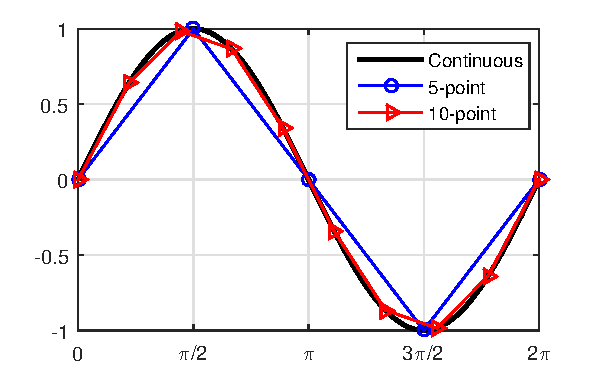
\includegraphics[width=0.55\textwidth]{spatial_discretization.pdf}\\
	\caption{Example of different spatial discretization}\label{fig:spatial_discretization}
\end{figure}

The value of $ \lambda $ is different for different frequencies:
\[
\lambda = V_S/f
\]
where $ f $ is the frequency of the harmonic wave component, and $ V_S $ is the shear wave velocity of a specific layer. The default maximum frequency that SeismoSoil is set to resolve is 30~Hz, thus
\[
\Delta h \,\,[\mathrm{m}] = \frac{V_S\,\,[\mathrm{m/s}]}{300\,\mathrm{sec}^{-1}}
\]


Layers with smaller $ V_S $ will be discretized to finer sublayers. This process is done internally within SeismoSoil.

If the users have needs for simulating frequencies higher than 30~Hz, please contact the authors.




\subsubsection{Deconvolution of rock-outcrop motions}\label{sec:deconvolution}

Oftentimes, the rock-outcrop motions, or the ``reference station'' motions, are used as the input motion to calculate the response of the softer soil site (see Figure~\ref{fig:three-types-of-input-motions} on page~\pageref{fig:three-types-of-input-motions}). The rock has a low value of damping ratio, therefore using rock-outcrop motions as input motions is acceptable, but not exactly accurate. If the rock properties (i.e., $V_S$, damping ratio) are known, and also the depth of the soil deposit is known, the users are advised to deconvolve (i.e., ``propagate downwards'') the rock-outcrop motion to the rock-soil interface, and then use the motion as the input incident motion. This results in a slightly stronger input motion, because the energy loss within the rock is accounted for and corrected.




\bibliographystyle{agufull04}
\addcontentsline{toc}{section}{\refname}\bibliography{seismosoil_ref}


\end{document} 